% Options for packages loaded elsewhere
\PassOptionsToPackage{unicode}{hyperref}
\PassOptionsToPackage{hyphens}{url}
%
\documentclass[
]{article}
\usepackage{amsmath,amssymb}
\usepackage{lmodern}
\usepackage{iftex}
\ifPDFTeX
  \usepackage[T1]{fontenc}
  \usepackage[utf8]{inputenc}
  \usepackage{textcomp} % provide euro and other symbols
\else % if luatex or xetex
  \usepackage{unicode-math}
  \defaultfontfeatures{Scale=MatchLowercase}
  \defaultfontfeatures[\rmfamily]{Ligatures=TeX,Scale=1}
\fi
% Use upquote if available, for straight quotes in verbatim environments
\IfFileExists{upquote.sty}{\usepackage{upquote}}{}
\IfFileExists{microtype.sty}{% use microtype if available
  \usepackage[]{microtype}
  \UseMicrotypeSet[protrusion]{basicmath} % disable protrusion for tt fonts
}{}
\makeatletter
\@ifundefined{KOMAClassName}{% if non-KOMA class
  \IfFileExists{parskip.sty}{%
    \usepackage{parskip}
  }{% else
    \setlength{\parindent}{0pt}
    \setlength{\parskip}{6pt plus 2pt minus 1pt}}
}{% if KOMA class
  \KOMAoptions{parskip=half}}
\makeatother
\usepackage{xcolor}
\IfFileExists{xurl.sty}{\usepackage{xurl}}{} % add URL line breaks if available
\IfFileExists{bookmark.sty}{\usepackage{bookmark}}{\usepackage{hyperref}}
\hypersetup{
  pdftitle={Spatial Analysis Severe Stigmatising Skin NTDs in Liberia},
  pdfauthor={Lucas Sempé},
  hidelinks,
  pdfcreator={LaTeX via pandoc}}
\urlstyle{same} % disable monospaced font for URLs
\usepackage[margin=1in]{geometry}
\usepackage{longtable,booktabs,array}
\usepackage{calc} % for calculating minipage widths
% Correct order of tables after \paragraph or \subparagraph
\usepackage{etoolbox}
\makeatletter
\patchcmd\longtable{\par}{\if@noskipsec\mbox{}\fi\par}{}{}
\makeatother
% Allow footnotes in longtable head/foot
\IfFileExists{footnotehyper.sty}{\usepackage{footnotehyper}}{\usepackage{footnote}}
\makesavenoteenv{longtable}
\usepackage{graphicx}
\makeatletter
\def\maxwidth{\ifdim\Gin@nat@width>\linewidth\linewidth\else\Gin@nat@width\fi}
\def\maxheight{\ifdim\Gin@nat@height>\textheight\textheight\else\Gin@nat@height\fi}
\makeatother
% Scale images if necessary, so that they will not overflow the page
% margins by default, and it is still possible to overwrite the defaults
% using explicit options in \includegraphics[width, height, ...]{}
\setkeys{Gin}{width=\maxwidth,height=\maxheight,keepaspectratio}
% Set default figure placement to htbp
\makeatletter
\def\fps@figure{htbp}
\makeatother
\setlength{\emergencystretch}{3em} % prevent overfull lines
\providecommand{\tightlist}{%
  \setlength{\itemsep}{0pt}\setlength{\parskip}{0pt}}
\setcounter{secnumdepth}{5}
\newlength{\cslhangindent}
\setlength{\cslhangindent}{1.5em}
\newlength{\csllabelwidth}
\setlength{\csllabelwidth}{3em}
\newlength{\cslentryspacingunit} % times entry-spacing
\setlength{\cslentryspacingunit}{\parskip}
\newenvironment{CSLReferences}[2] % #1 hanging-ident, #2 entry spacing
 {% don't indent paragraphs
  \setlength{\parindent}{0pt}
  % turn on hanging indent if param 1 is 1
  \ifodd #1
  \let\oldpar\par
  \def\par{\hangindent=\cslhangindent\oldpar}
  \fi
  % set entry spacing
  \setlength{\parskip}{#2\cslentryspacingunit}
 }%
 {}
\usepackage{calc}
\newcommand{\CSLBlock}[1]{#1\hfill\break}
\newcommand{\CSLLeftMargin}[1]{\parbox[t]{\csllabelwidth}{#1}}
\newcommand{\CSLRightInline}[1]{\parbox[t]{\linewidth - \csllabelwidth}{#1}\break}
\newcommand{\CSLIndent}[1]{\hspace{\cslhangindent}#1}
\ifLuaTeX
  \usepackage{selnolig}  % disable illegal ligatures
\fi

\title{Spatial Analysis Severe Stigmatising Skin NTDs in Liberia}
\usepackage{etoolbox}
\makeatletter
\providecommand{\subtitle}[1]{% add subtitle to \maketitle
  \apptocmd{\@title}{\par {\large #1 \par}}{}{}
}
\makeatother
\subtitle{Years 2019-2021}
\author{Lucas Sempé}
\date{}

\begin{document}
\maketitle

{
\setcounter{tocdepth}{2}
\tableofcontents
}
\hypertarget{analysis-of-cases-2019---2021}{%
\subsection{Analysis of cases 2019 - 2021}\label{analysis-of-cases-2019---2021}}

\hypertarget{raw-cases}{%
\subsubsection{Raw cases}\label{raw-cases}}

Liberia is one of the first countries in the world to develop a national integrated approach to managing SSSDs, namely, lymphatic filariasis (LF), leprosy, Buruli ulcer (BU), yaws, hydrocele (HC) and onchocerciasis. This means managing diseases with signs on the skin, through a combined approach at the local level.

The Ministry of Health of Liberia has 1,113 cases of 5 SSSDs: BU, HC, Leprosy, LF and Yaws from 2019 to 2021. BU represents 44\% of total cases (488), followed by HC (21\% as in 239 cases), Leprosy (16\% as in 179 cases), LF with 167 cases (15\% of total) and 40 cases of yaws (4\%). Table \ref{tab:casyear}) shows disaggregated figures per year and disease, where we observe a decrease in the numbers of detected cases of BU (from 197 to 122), an increase in the cases of HC, LF and Yaws (up to 94, 112 and 40 in 2021), while leprosy has an oscillating behaviour over time.

\begin{table}

\caption{\label{tab:casyear}Number of cases per year - SSSDs}
\centering
\begin{tabular}[t]{l|r|r|r|r|r|r}
\hline
Year & BU & HC & Leprosy & LF & Yaws & Total\\
\hline
2019 & 197 & 55 & 52 & 32 & 0 & 336\\
\hline
2020 & 169 & 90 & 82 & 23 & 12 & 376\\
\hline
2021 & 122 & 94 & 45 & 112 & 28 & 401\\
\hline
Total & 488 & 239 & 179 & 167 & 40 & 1113\\
\hline
\end{tabular}
\end{table}

Figure \ref{fig:cases-year} portrays the number of detected cases across years 2019 to 2021 for the 5 diseases. It is possible to observe geographical patterns for BU (with the majority of cases found in the North and East of the country) and Leprosy (with cases found in the middle and center-south of the country). For the other diseases,

\begin{figure}
\centering
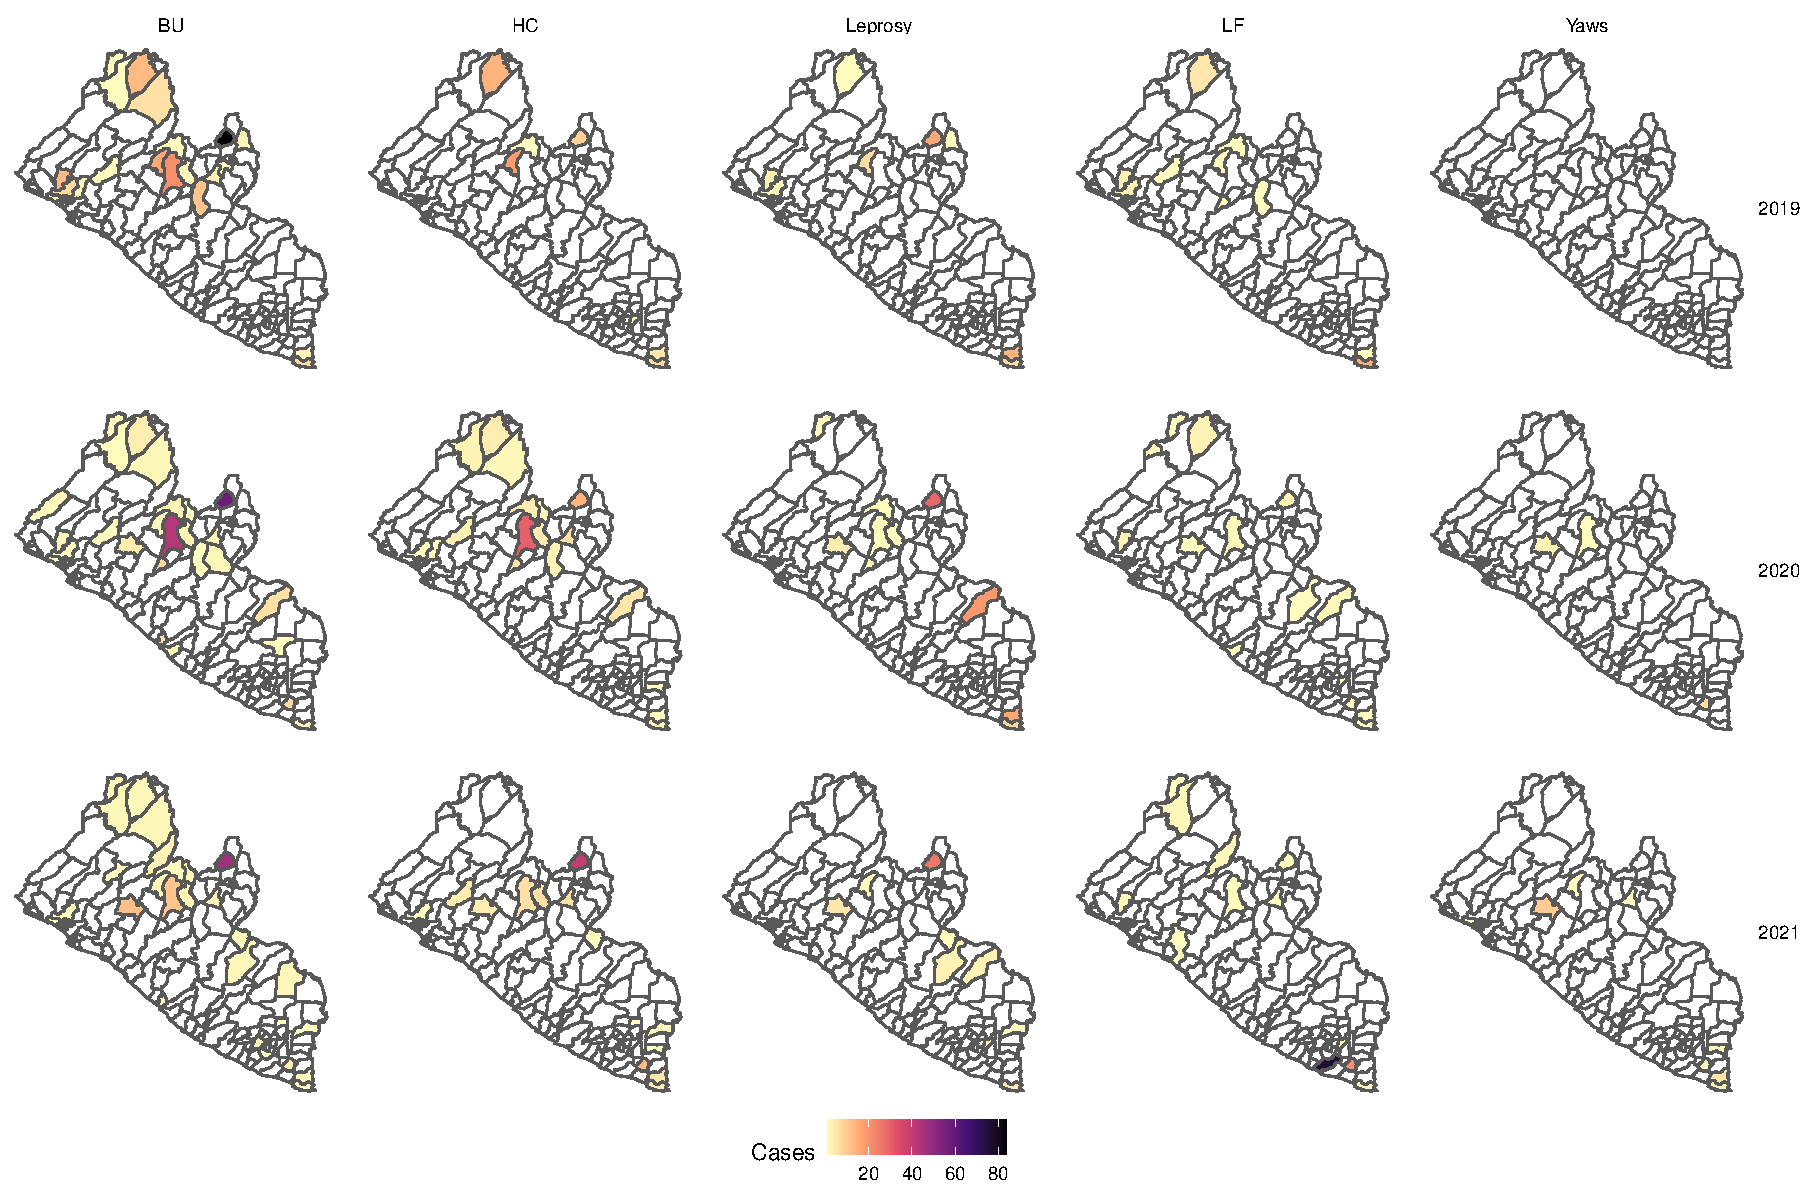
\includegraphics{_main_files/figure-latex/cases-year-1.pdf}
\caption{\label{fig:cases-year}Cases per disease and year over time}
\end{figure}

Over the period, any of the 5 aforementioned diseases were detected in 46 districts out of the 136 districts (34\% of the total number of districts in the country), where only in 5 districts all diseases were found, while 8 districts have detected cases of 4 diseases, 11 districts detected cases of 3 diseases, 10 districts detected cases of 2 diseases and 12 districts detected only 1 disease (see Figure \ref{fig:prop1}).

\textbf{Karsor/Laura: does it make sense to expect an increase on the identification of more diseases in the same district?}

\begin{figure}
\centering
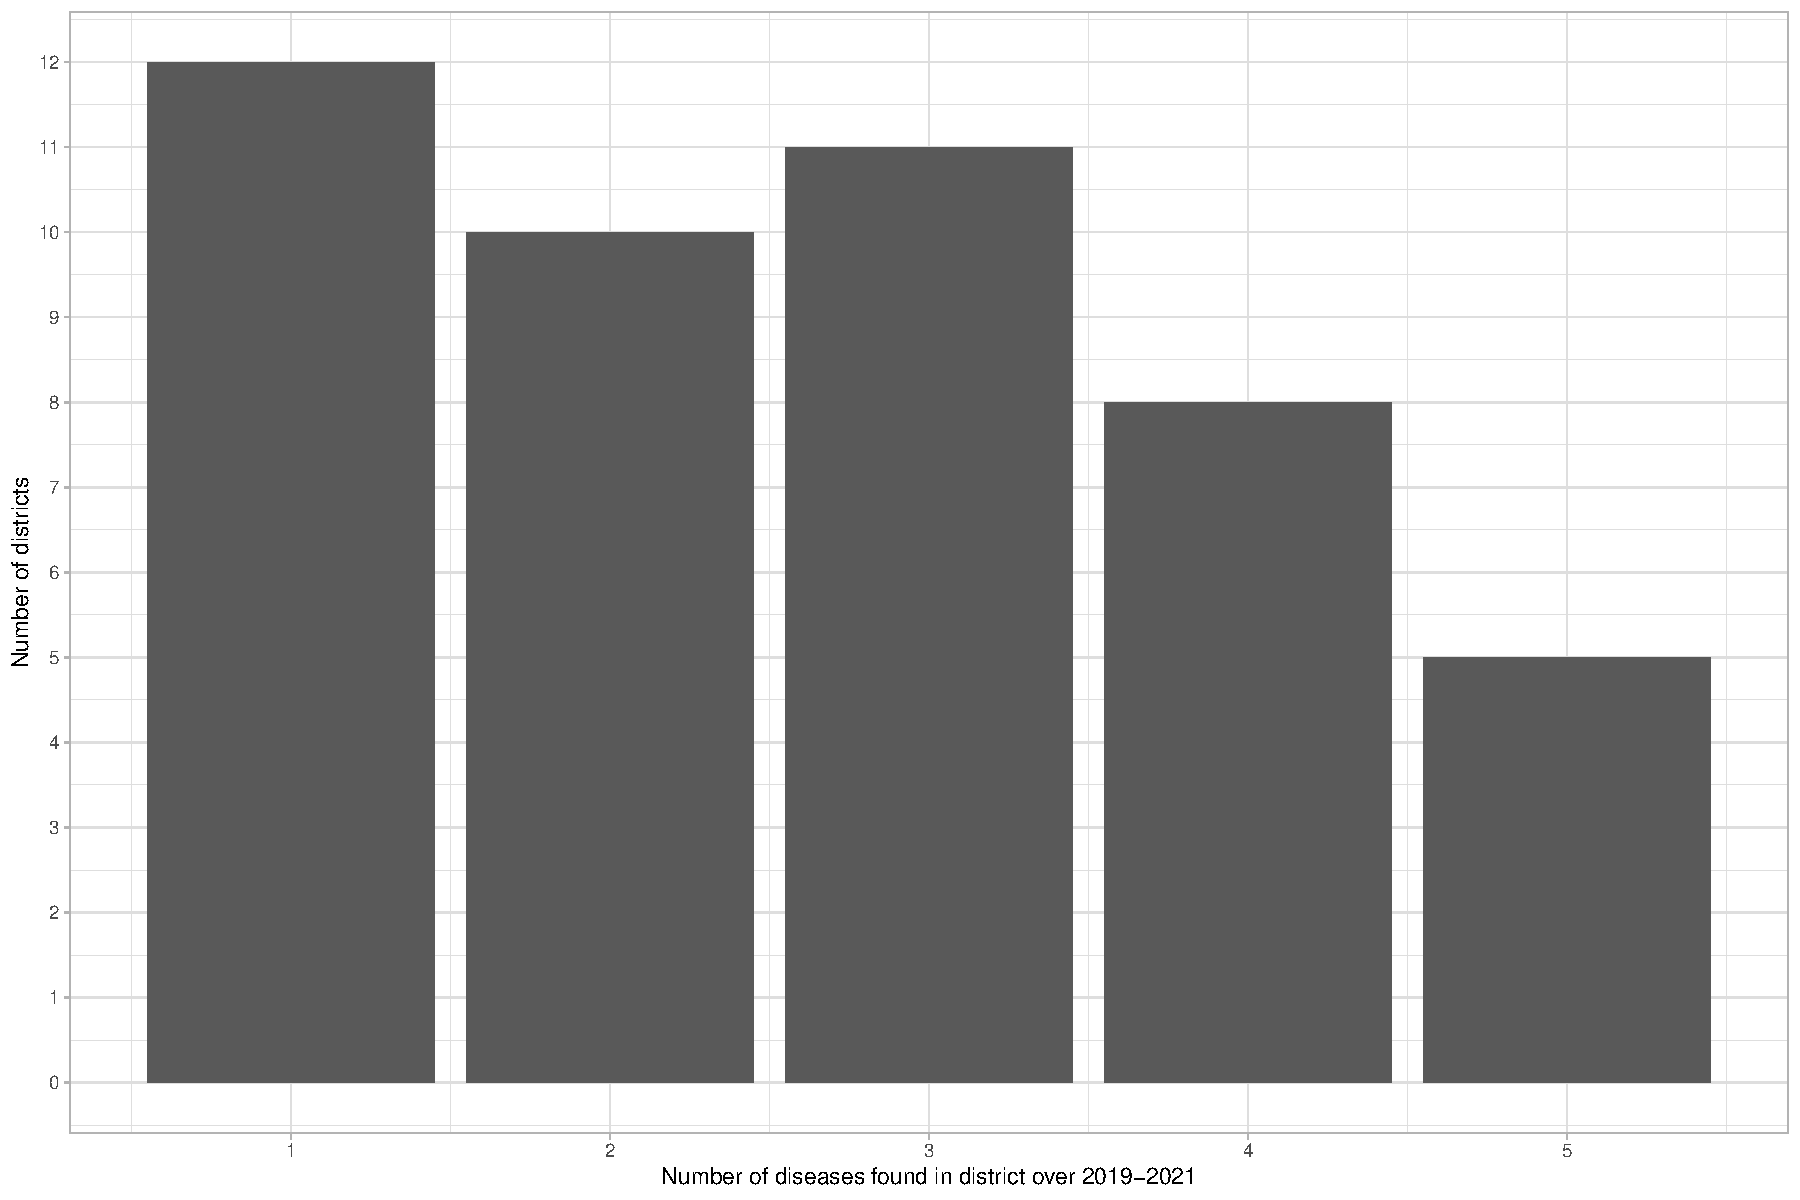
\includegraphics{_main_files/figure-latex/prop1-1.pdf}
\caption{\label{fig:prop1}Number of districts were one or more diseases were detected over the period 2019 to 2021}
\end{figure}

Figure \ref{fig:saniquele}) shows the proportion of the total cases per year and disease found in the district of Sanniquellie Mahn in Nimba, where a national reference center is based. BU cases oscillates between 34\% and 43\% of the total, while HC and Leprosy show an important increase in year 2021, reaching 43\% and 58\%, respectively. LF shows lower values, reaching 13\% in 2020 and there were no identified cases of Yaws.

\textbf{Karsor: why the increase in HC/Leprosy in 2021?}

\textbf{Karsor/Laura: is it possible to know from how far people go there? (so we can estimate the endemic areas and not the point of treatment)}

\textbf{Karsor: is correct to expect that this \% goes down with IC across counties?}

\begin{figure}
\centering
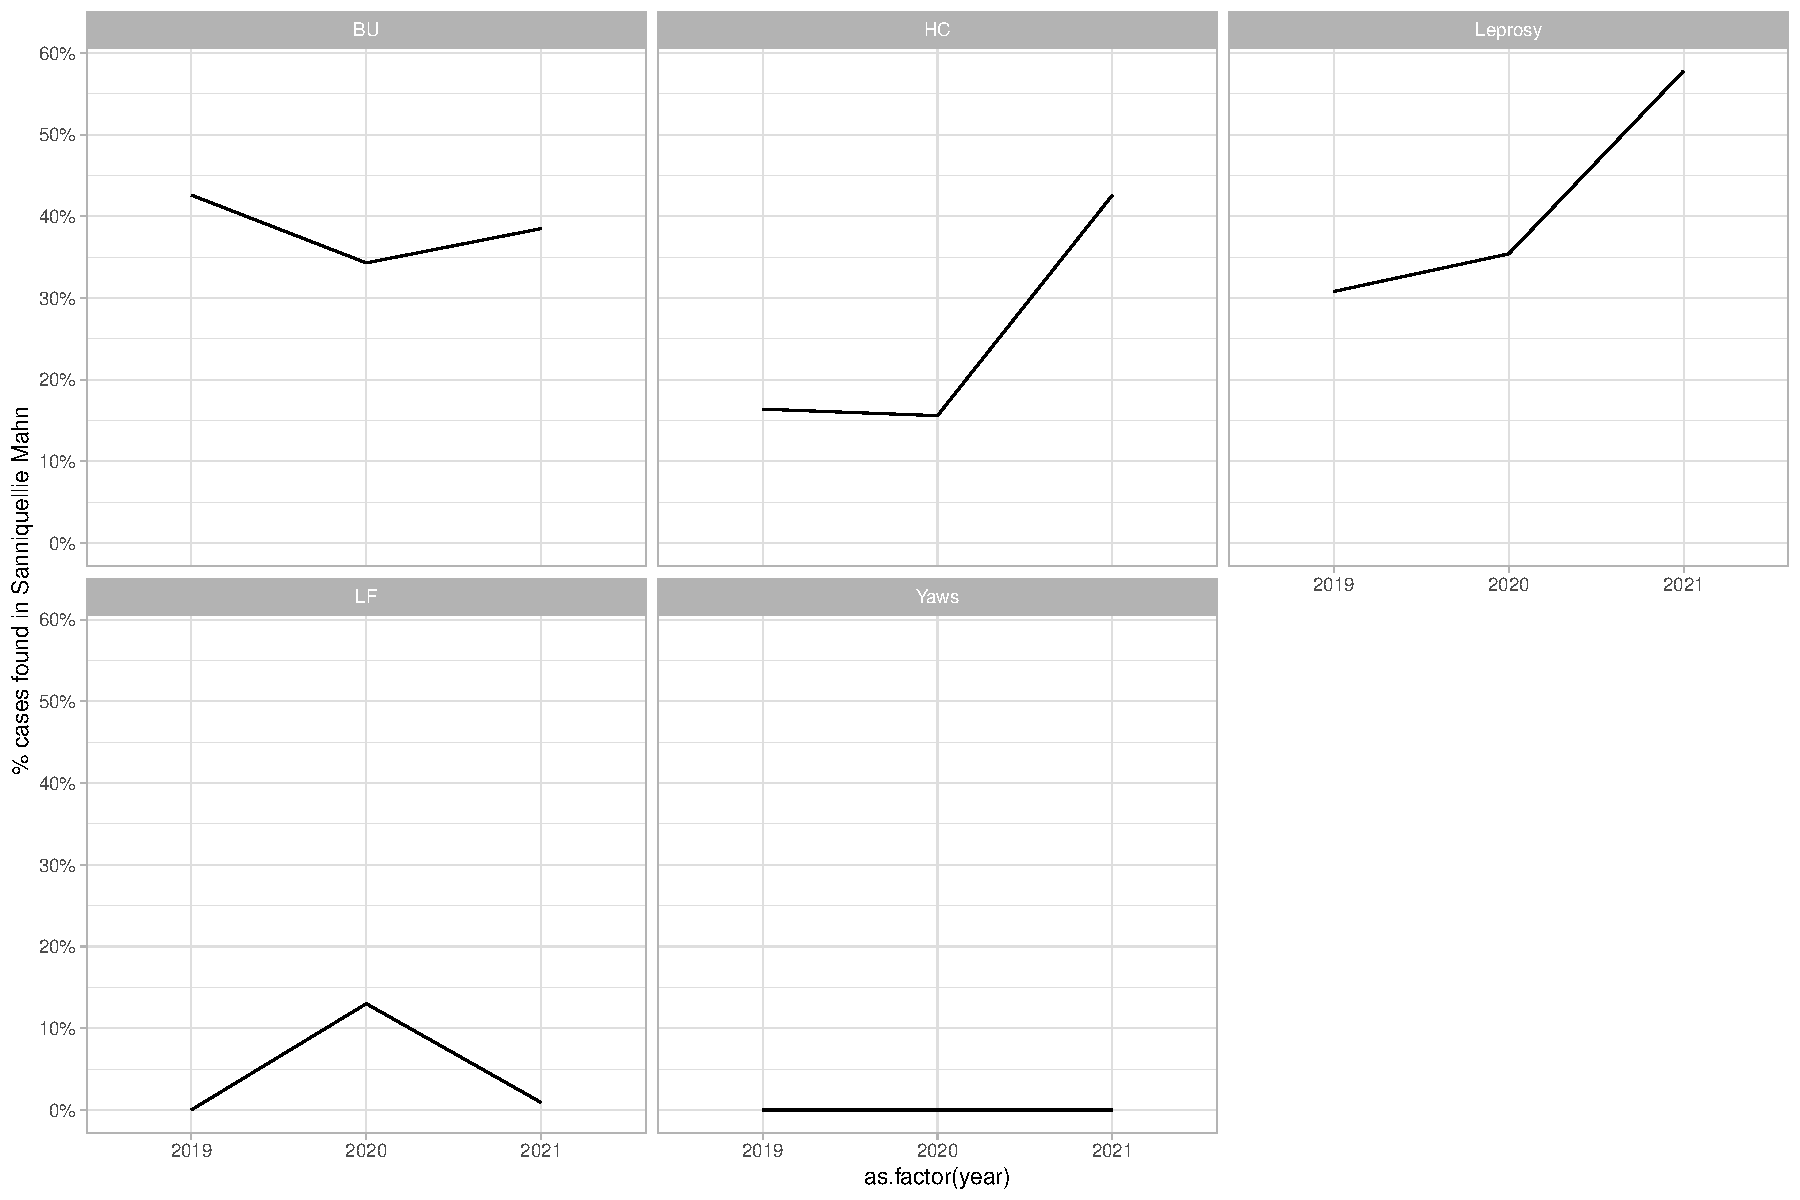
\includegraphics{_main_files/figure-latex/saniquele-1.pdf}
\caption{\label{fig:saniquele}Proportion of cases found in Sanniquellie Mahn by disease and year}
\end{figure}

\hypertarget{analysis-and-comparison-with-other-countries}{%
\subsubsection{Analysis and comparison with other countries}\label{analysis-and-comparison-with-other-countries}}

In the case of \textbf{\emph{BU}}, we find national rates between 0.4 and 0.7 per 10,000 inhabitants across years. The highest rates are found in Trenbo, Grand Kru, in 2020 (36.8 cases per 10,000 inhabitants) followed by Sanniquellie Mahn in 2019 and 2020 (24.1 cases per 10,000 and 16.6 cases per 10,000). As a comparison, Simpson et al. (2019) reviewed different prevalence studies in West Africa finding rates between 3.2 to 26.9 cases per 10,000. See table in Appendix.

\textbf{Karsor: Trenbo consistently has higher rates. Is there a plausible explanation?}

In the case of \textbf{\emph{LF}}, we find rates between 0.05 and 1.2 per 10,000 inhabitants across years. However, the rate in 2021 is 1,300 times higher than in 2020. This raise is produced by Trenbo and Barclayville in Grand Kru, with rates of 110 and 50.6 cases in 10,000 people.

\textbf{Karsor: Trenbo and Barclayville suggest 1 in 100 and 1 in 200 have LF. Is that feasible?}

As a comparison, a Bayesian geospatial estimation by the Local Burden of Disease 2019 Neglected Tropical Diseases Collaborators (Cromwell et al. 2020) suggests 11.1\% of prevalence in Liberia, with districts in Nimba with an estimated prevalence over 30\% where many areas in the country are unlikely to be below the 2\% threshold of prevalence (posterior probability \textless5\% of not occurring). See appendix for estimations per district.

\textbf{Karsor/Laura: Is this feasible?}

In the case of \textbf{\emph{Leprosy}}, we find stable rates between 0.08 and 0.16 per 10,000 inhabitants across years. Besides Sanniquellie Mahn (rates oscillate between 4.6 in 2019 and 8.31 in 2020), other districts with higher rates are Kokoyah, Bong (4.06 cases in 10,000) and Tchien, in Grand Gedeh (3.7 cases in 10,000).

As a comparison, WHO compiled in 2016 prevalence and new cases for the world (WHO 2016), where Africa shows a prevalence rate of .3 per 10,000 and 2 new cases per 100,000.

\textbf{Karsor/Laura: Liberia has on average 50\% less detected cases than other countries. Does it make sense?}

In the case of \textbf{HC}, rates growth from .09 per 10,000 in 2019 to .7 per 10,000 in 2021, driven by cases found in Sanniquellie Mahn (40) and Trenbo (13). There was no available information in the literature to benchmark prevalence or newly detected cases.

\textbf{Karsor/Laura: Any data or source?}

Finally, in the case of \textbf{Yaws}, there were no cases registered in 2019, while in 2020 and 2021 rates grew from .09 per 10,000 in 2020 to .28 in 2021. The district of Trenbo, both in 2020 and 2021 show the highest ratios in the country, 5.3 and 36.8 per 10,000 respectively. In terms of raw cases, the district of Salala in Bong has the highest number (10 cases in 2021), followed by Pleebo/Sodoken in Maryland (5 cases in 2021) and Commonwealth in Grand Bassa (4 cases in 2021).

As a comparison, a recent systematic review finds the prevalence of active yaws lesions ranged from in tropical forests in Central Africa, including 9\% per in Cameroon, 11\% in the Central African Republic, 4·77\% in the Democratic Republic of the Congo, and 2·95\% in the Republic of Congo (Mitjà et al. 2015).

\textbf{Karsor/Laura: Does this data make sense?}

\hypertarget{integrated-case-management}{%
\subsection{Integrated case management}\label{integrated-case-management}}

The integrated case management intervention has been deployed across 5 counties: Bomi, Bong, Lofa, Maryland and Nimba (see Figure \ref{fig:ntd}).

\textbf{Karsor: is this map correct?}

\begin{figure}
\centering
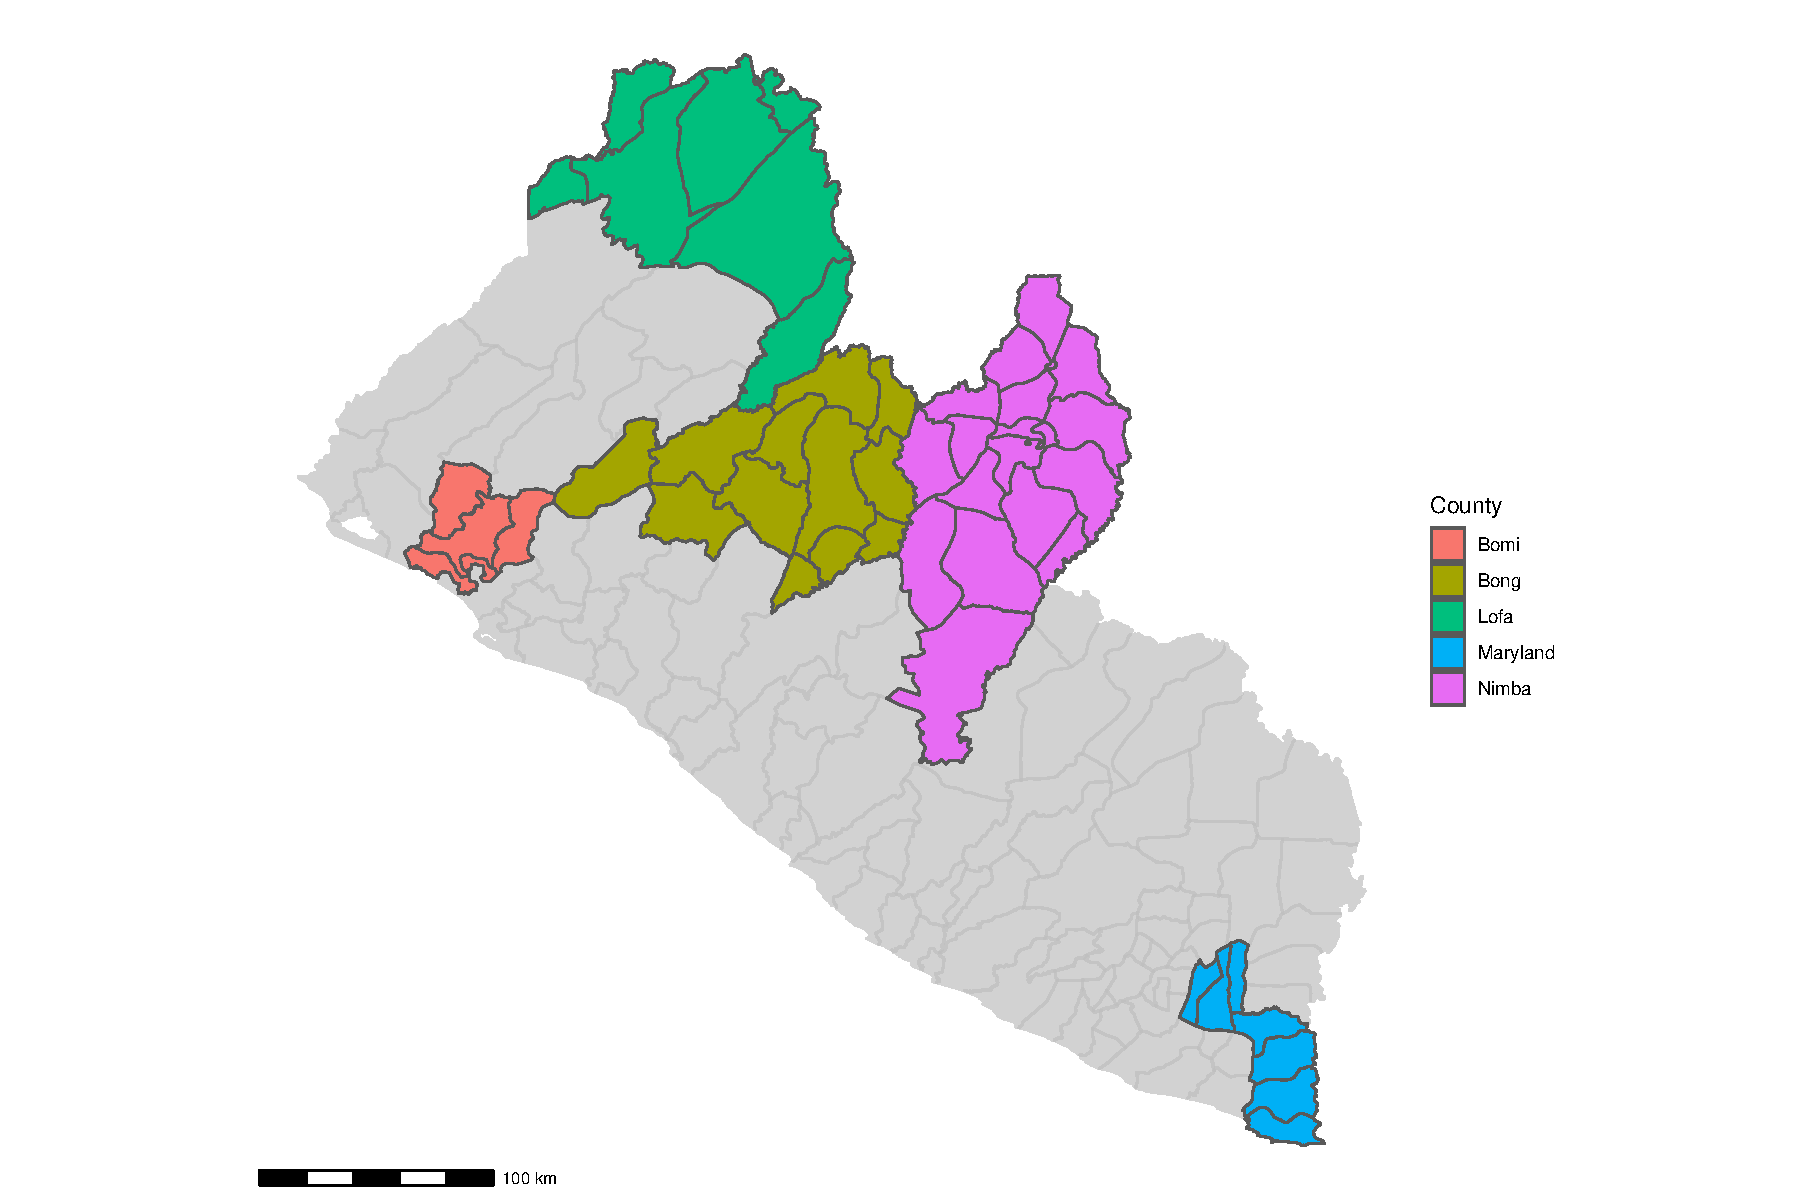
\includegraphics{_main_files/figure-latex/ntd-1.pdf}
\caption{\label{fig:ntd}Counties with NTDs integrated case management}
\end{figure}

Figures \ref{fig:cases-total-int} and \ref{fig:cases-total-not} show the total number of cases

\begin{figure}
\centering
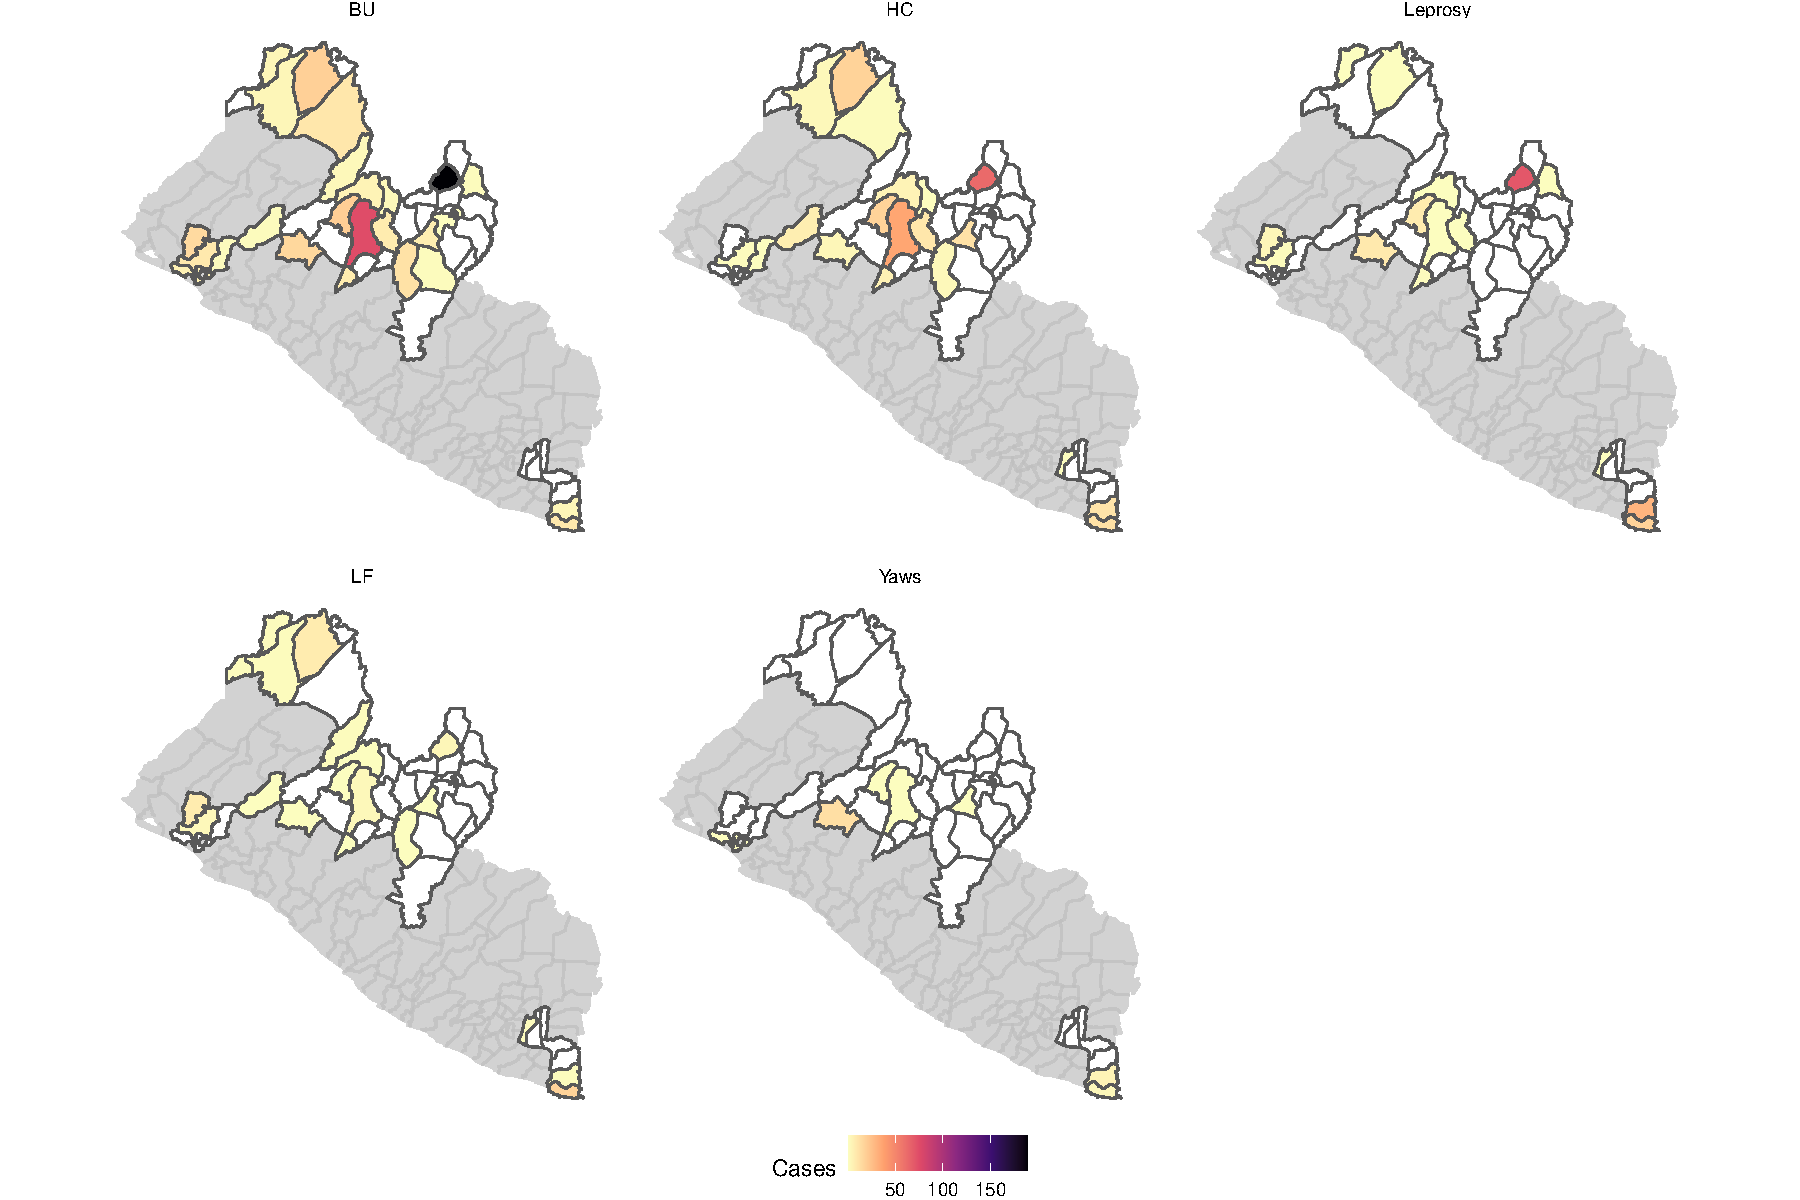
\includegraphics{_main_files/figure-latex/cases-total-int-1.pdf}
\caption{\label{fig:cases-total-int}Cases in IC districts - 2019-2021}
\end{figure}

\begin{figure}
\centering
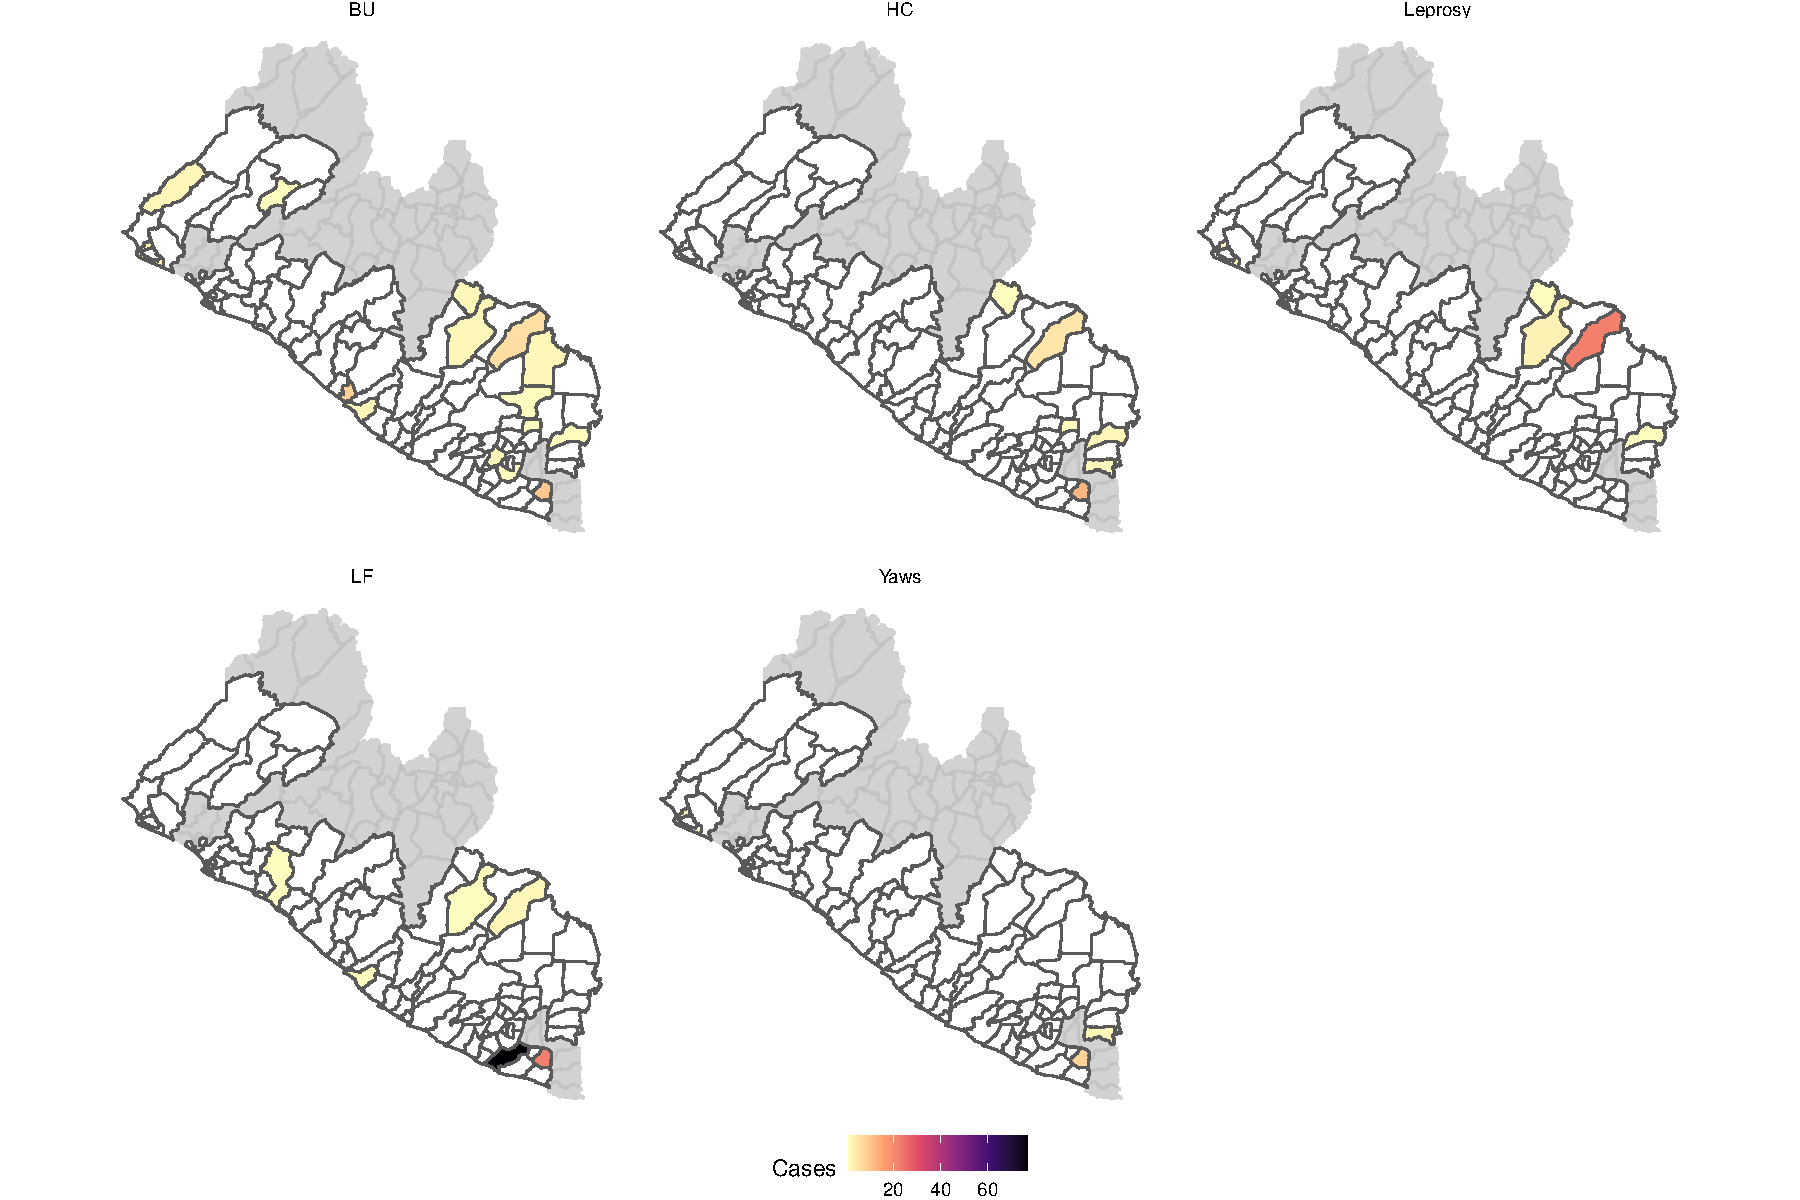
\includegraphics{_main_files/figure-latex/cases-total-not-1.pdf}
\caption{\label{fig:cases-total-not}Cases in nIC districts - 2019-2021}
\end{figure}

Figure \ref{fig:cas}) shows the evolution of the number of detected cases across two groups of counties, those implementing an integrated case management (IC) and those without an integrated care (nIC). We observe two different behaviors across diseases. In the first one (top row), the number of detected cases of Buruli Ulcer (BU), hydrocele (HC) and Leprosy is significantly higher in counties with integrated case management. The case of BU shows a 50\% decrease over time on IC counties from about 200 to 100. The case of LF is significantly different due to an intervention to actively detect cases in Barclayville (77 cases) and Trenbo (21 cases), both in Gran Kru county, in 2021.

\textbf{Karsor/Laura: is this intervention in Gran Kru correct?}

\begin{figure}
\centering
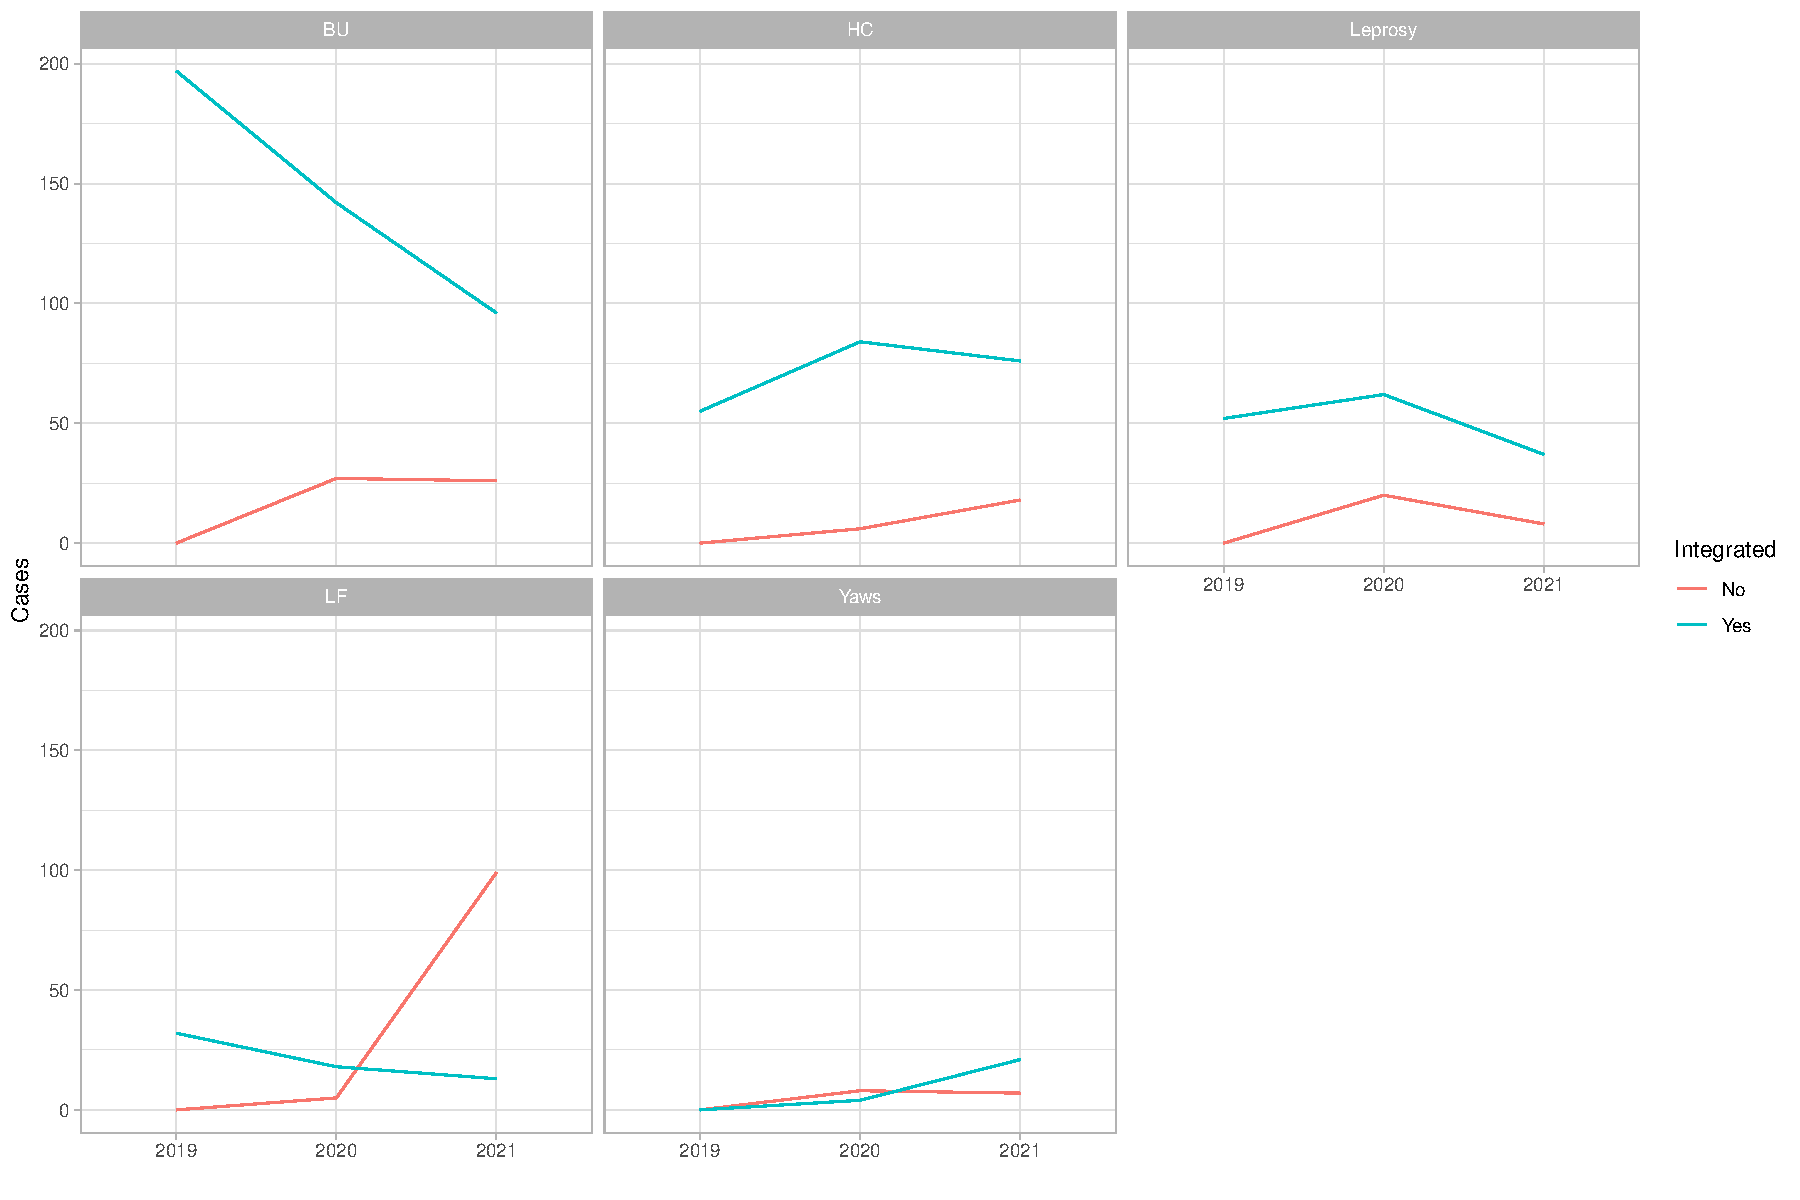
\includegraphics{_main_files/figure-latex/cas-1.pdf}
\caption{\label{fig:cas}Cases 2019-2021 by Integrated case management}
\end{figure}

Figure \ref{fig:prop2} presents the number of districts with 1 or more detected diseases over the period. Over the period, any of the 5 aforementioned diseases were detected in 27 districts out of the 47 districts (57.4\% of the total number of districts in the case management counties) and in 19 out of 80 districts without case management (21.3\% of correspondent districts). Only in 5 districts with integrated case management all 5 diseases were found, while in 6 districts with IC have detected cases of 4 diseases (in comparison to 2 in nIC); 7 districts with IC detected cases of 3 diseases, while only 4 nIC districts did the same; 6 districts with IC detected cases of 2 diseases, while only 4 nIC districts did the same. Finally, the number of districts which detected only 1 disease is higher in nIC areas (9) compared to 3 districts with IC detecting only 1 disease.

\begin{figure}
\centering
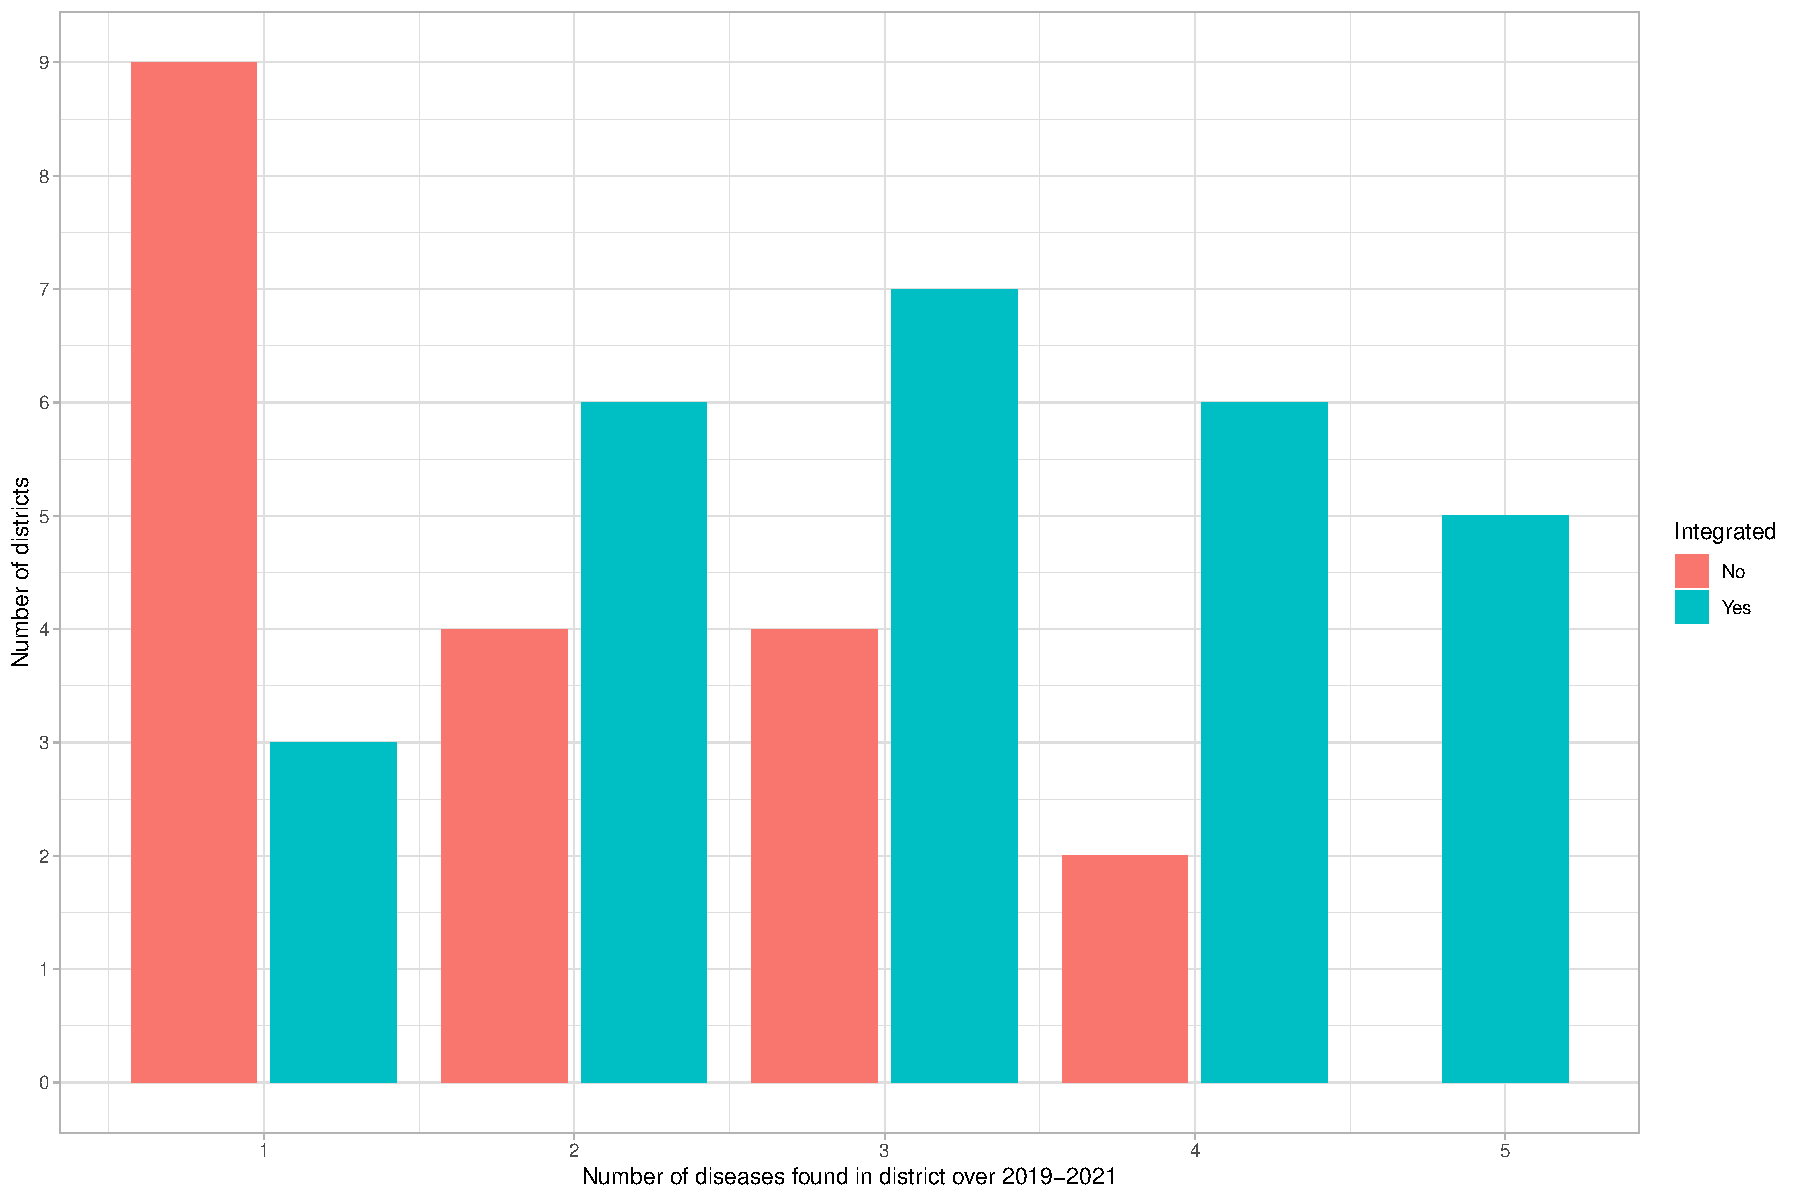
\includegraphics{_main_files/figure-latex/prop2-1.pdf}
\caption{\label{fig:prop2}Number of districts were one or more diseases were detected over the period 2019 to 2021 by Integrated Case management}
\end{figure}

Figure \ref{fig:rat}) shows the evolution of the number of detected cases per 10,000 inhabitants across both groups of counties. The analytic scenario is different from the raw count presented in Figure \ref{fig:cas}. We only observe a consistent higher ratio of IC counties in the case of Leprosy, while in BU and Yaws values are similar across groups. In the case of HC and LF, we observe that nIC counties show higher ratios in 2021.

\begin{figure}
\centering
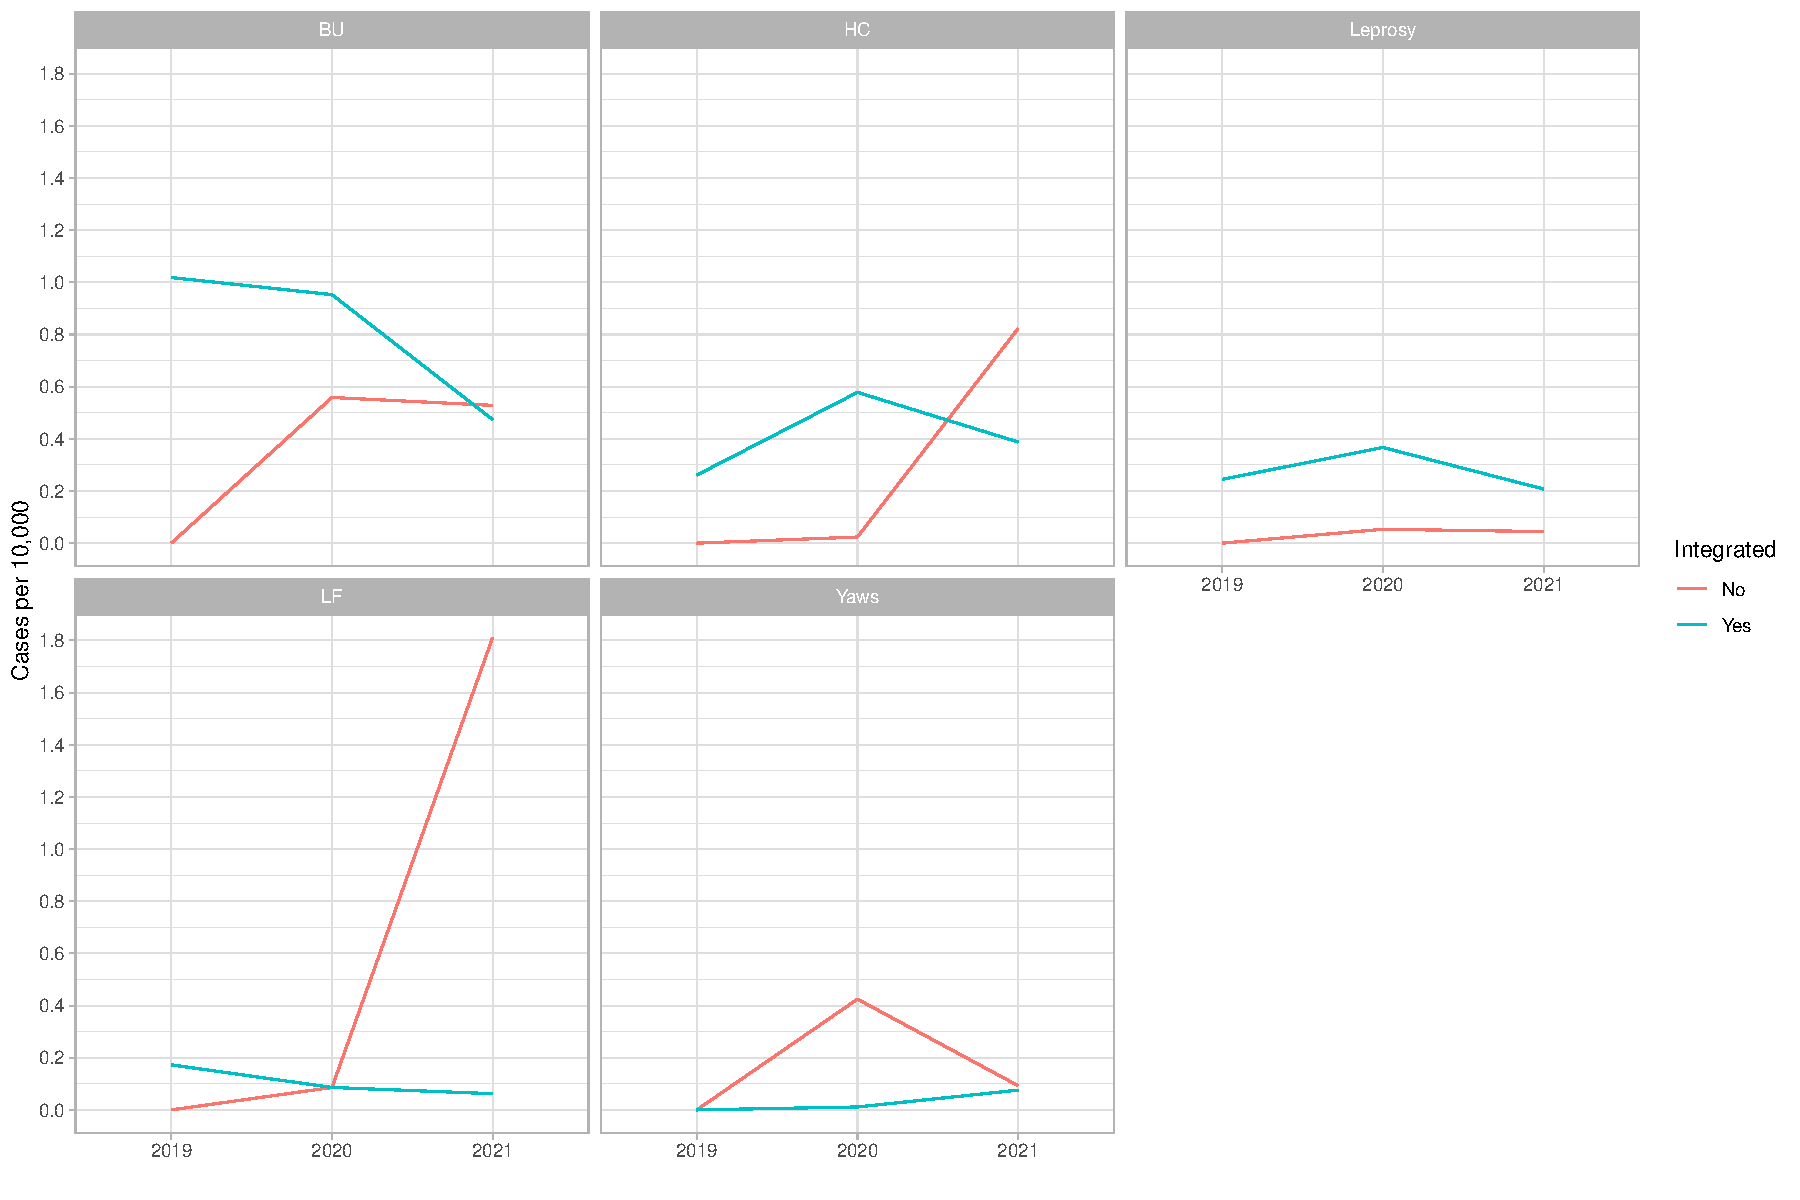
\includegraphics{_main_files/figure-latex/rat-1.pdf}
\caption{\label{fig:rat}Ratio 2019-2021 by Integrated case management}
\end{figure}

\hypertarget{inferential-analysis-spatial-autocorrelation-and-spatial-regressions}{%
\subsection{Inferential analysis: spatial autocorrelation and spatial regressions}\label{inferential-analysis-spatial-autocorrelation-and-spatial-regressions}}

\begin{figure}
\centering
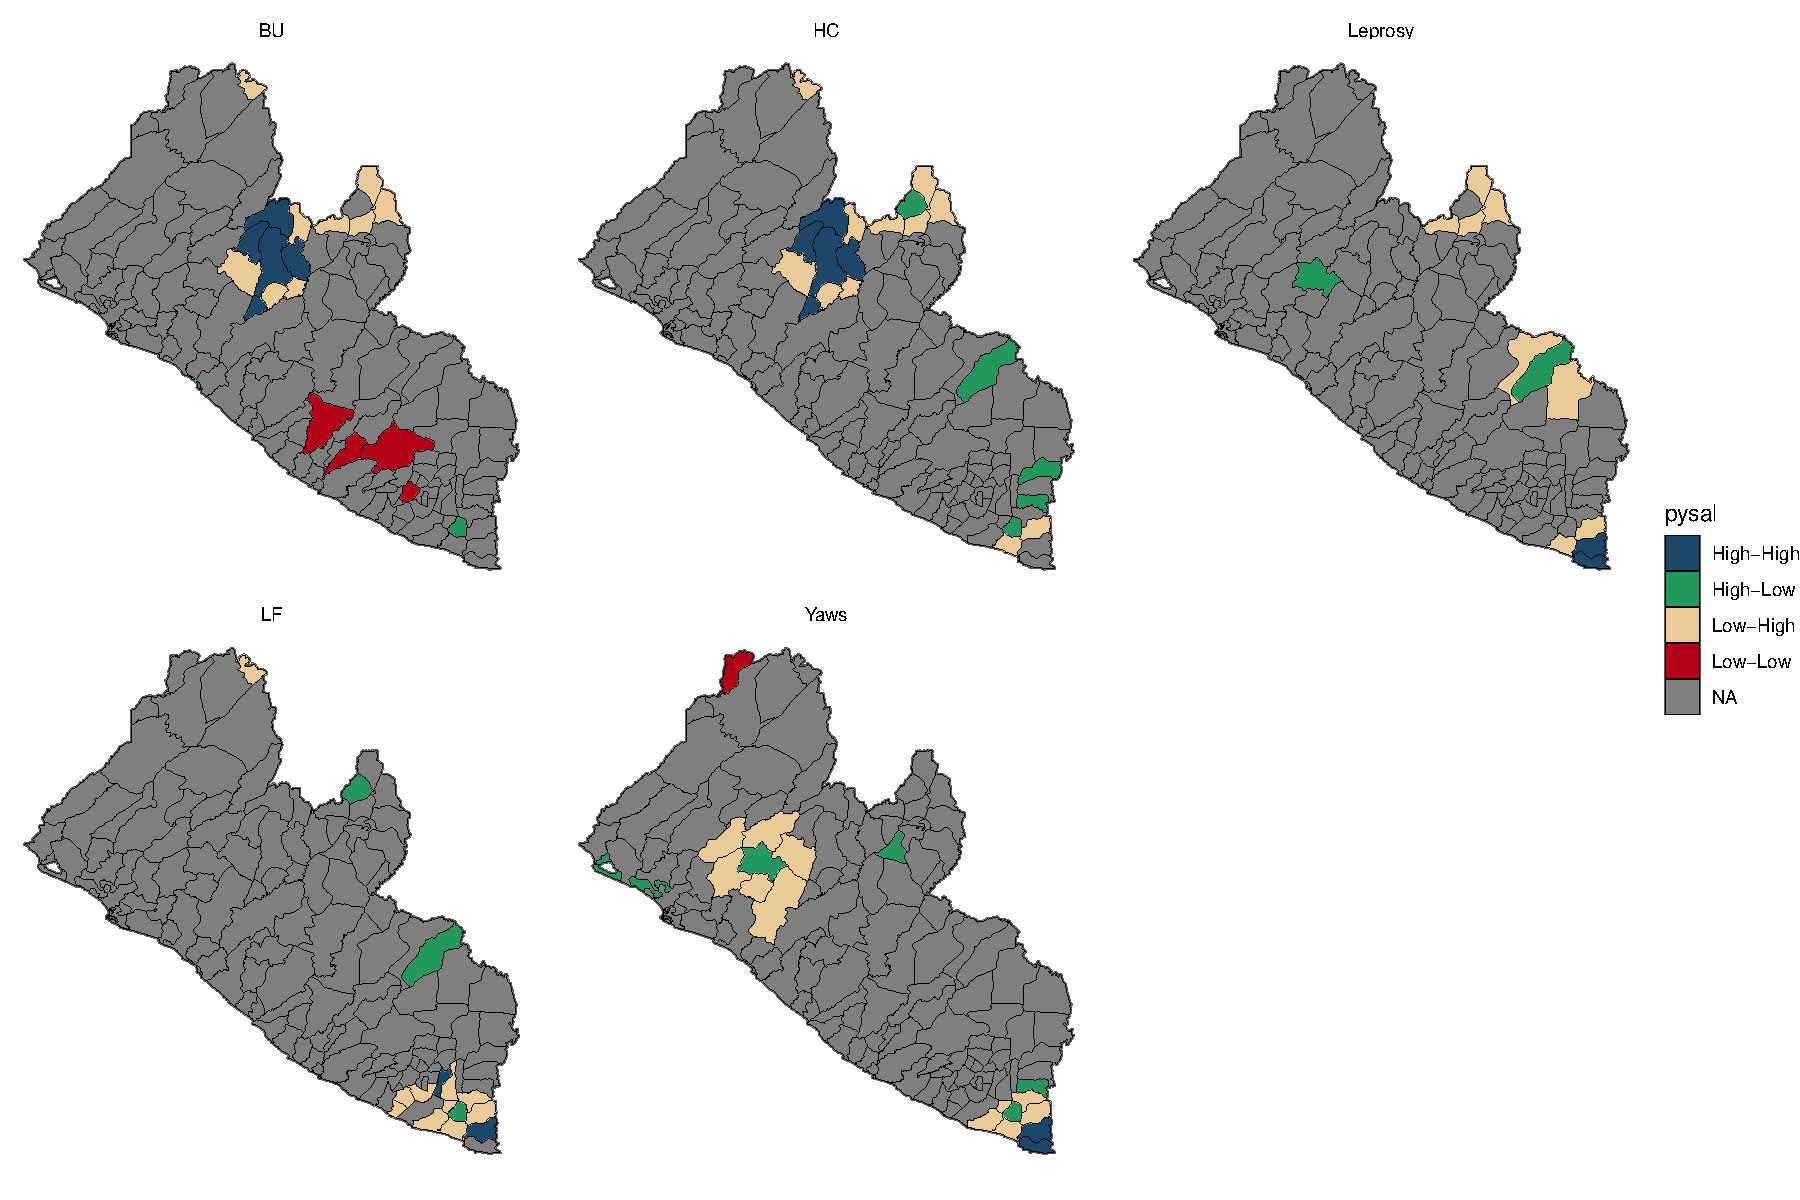
\includegraphics{_main_files/figure-latex/moran-1.pdf}
\caption{\label{fig:moran}Local Moran test}
\end{figure}

\begin{figure}
\centering
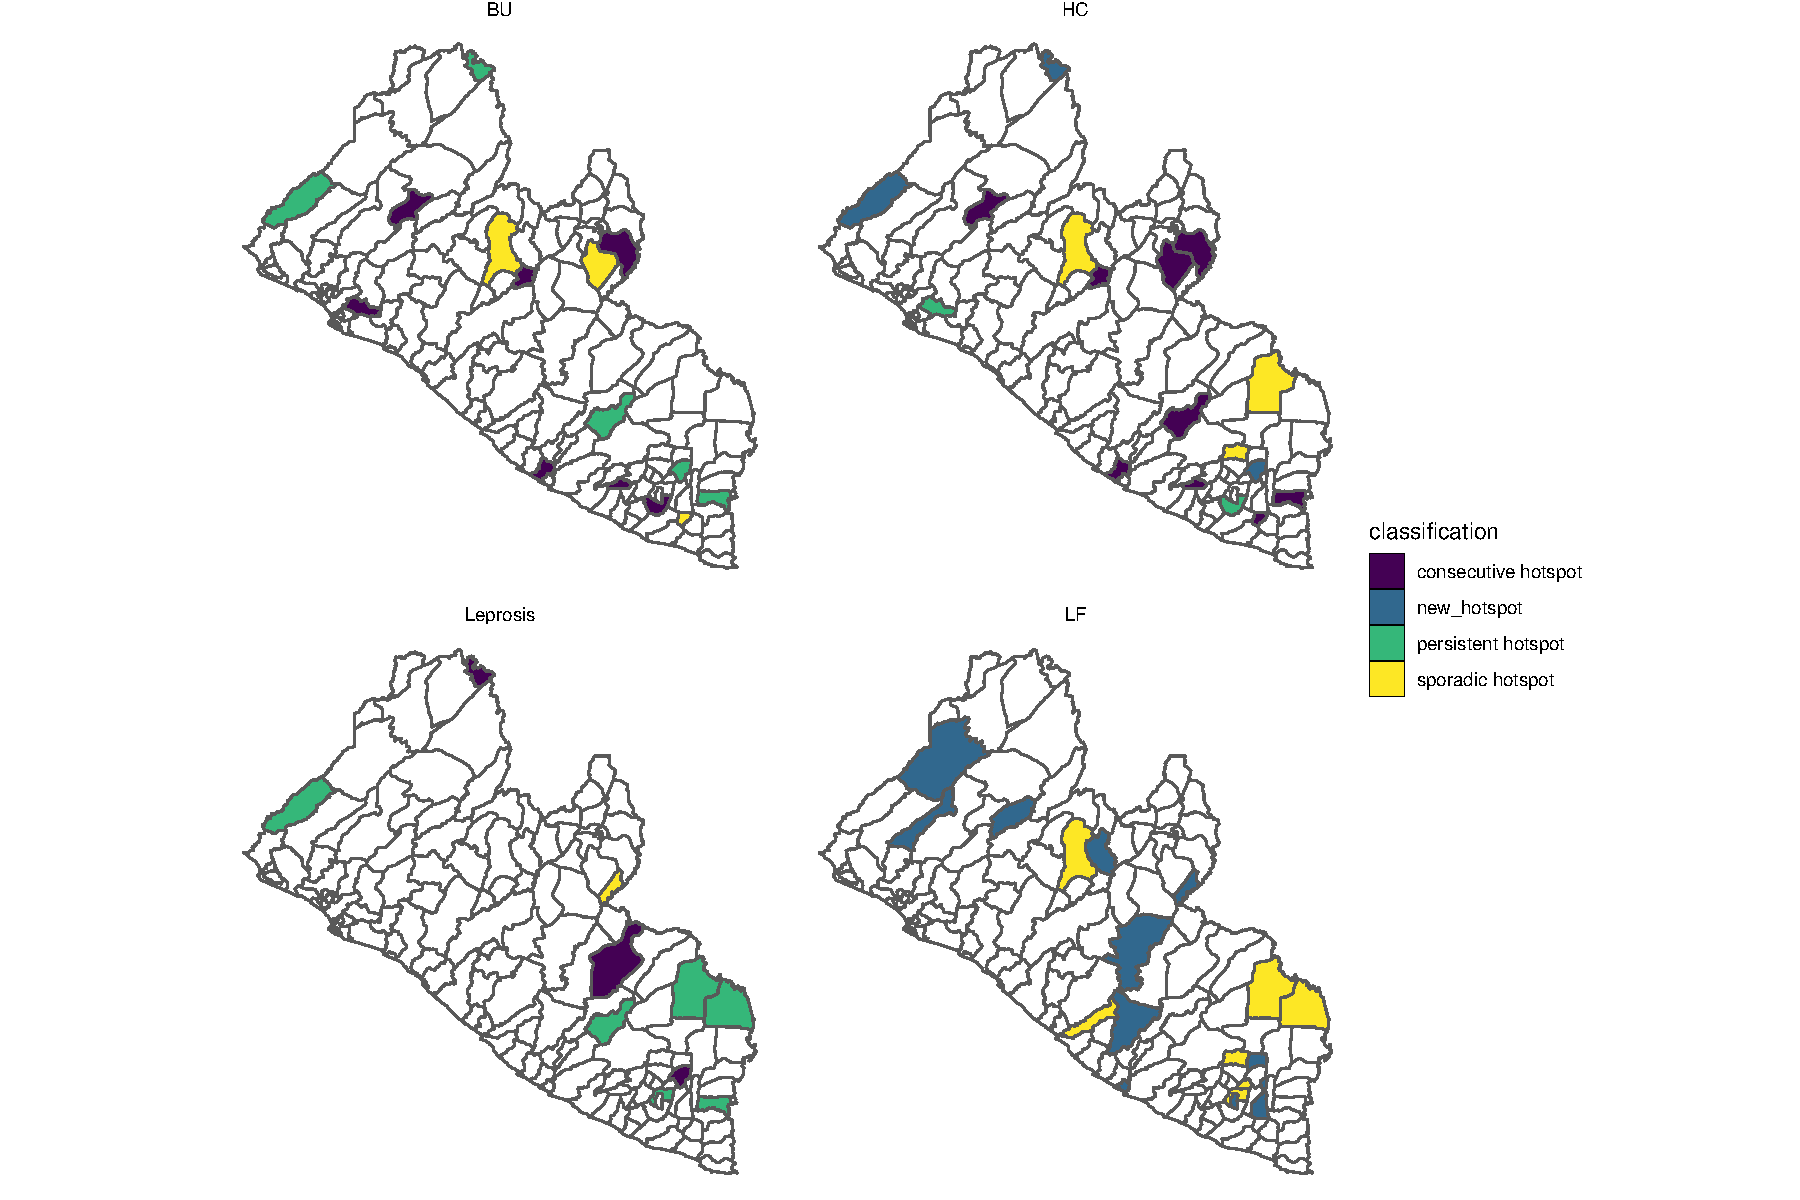
\includegraphics{_main_files/figure-latex/ehs-1.pdf}
\caption{\label{fig:ehs}Emergent hotspots analysis}
\end{figure}

\begin{figure}
\centering
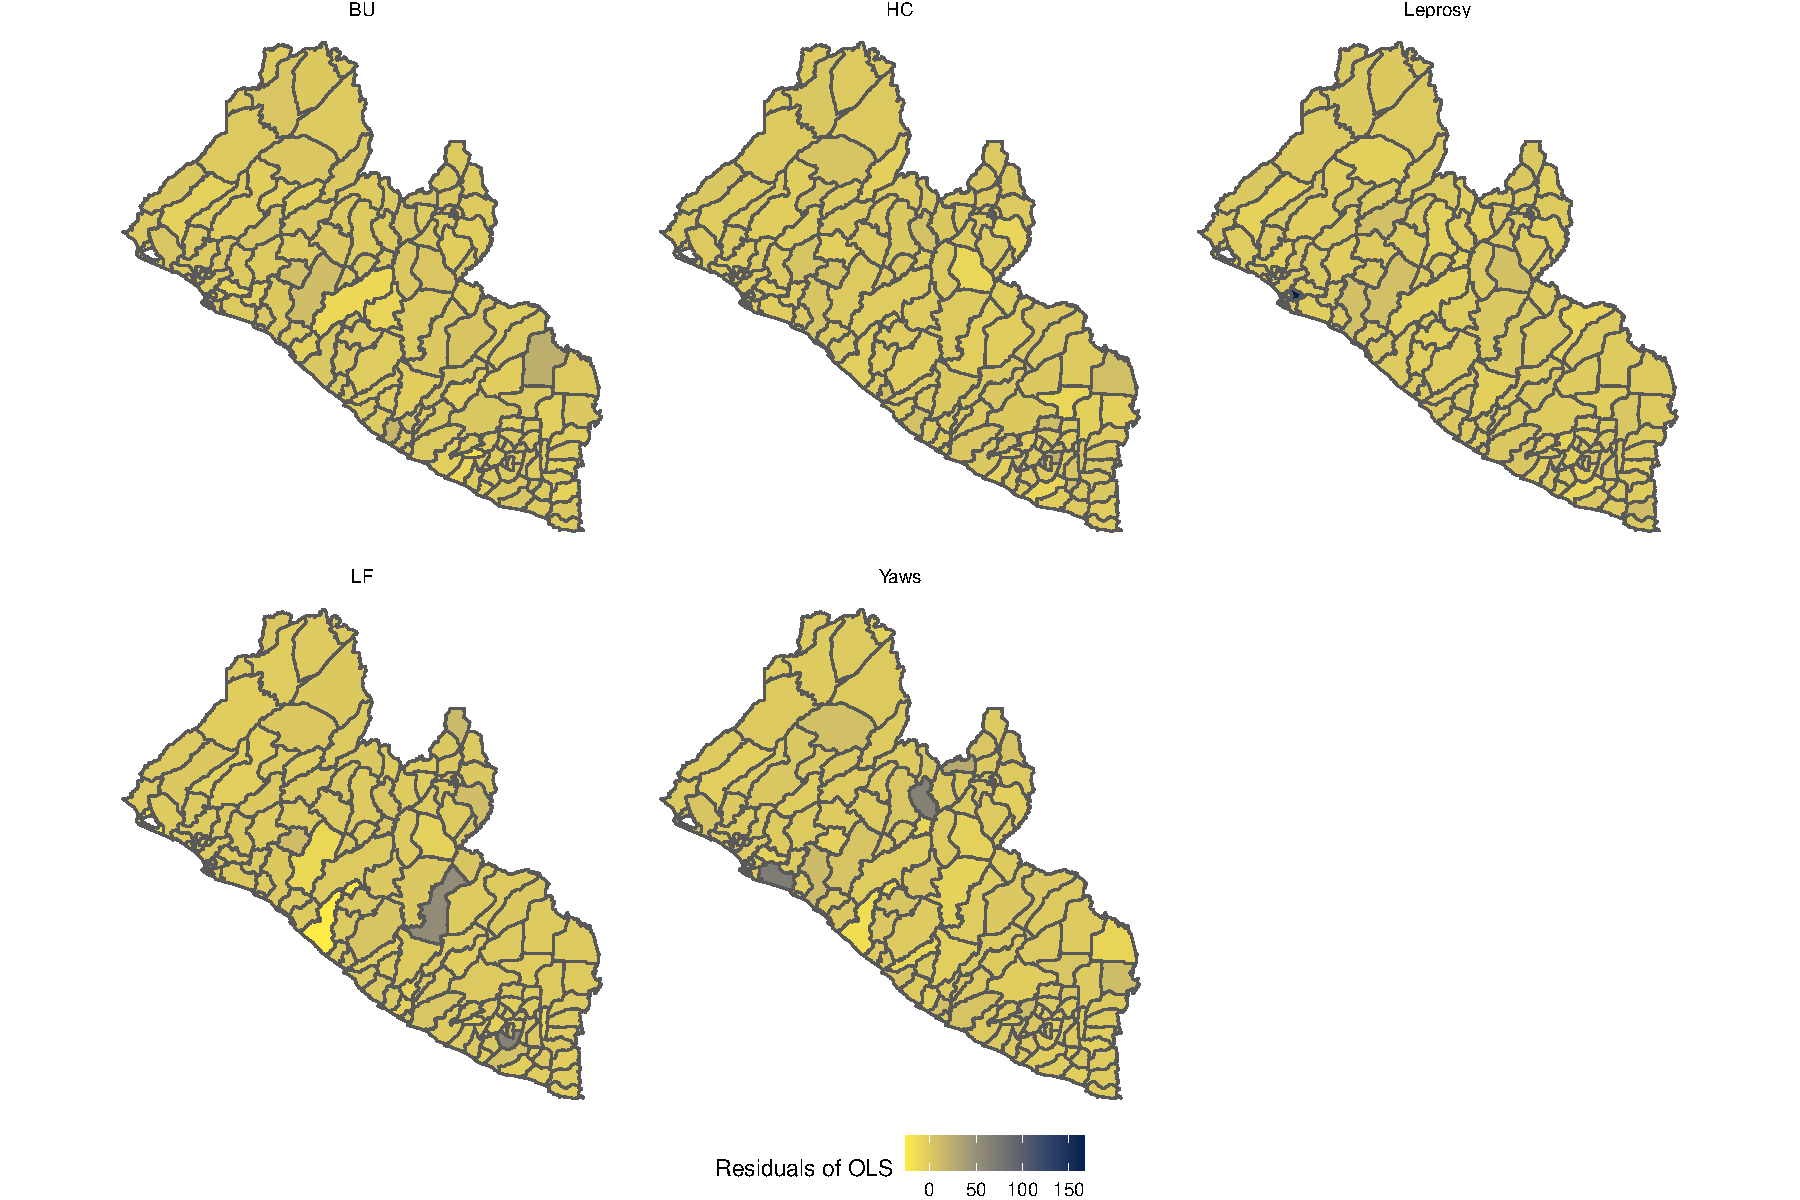
\includegraphics{_main_files/figure-latex/residuals-1.pdf}
\caption{\label{fig:residuals}Residuals OLS regression on number of cases}
\end{figure}

\hypertarget{references}{%
\subsection{References}\label{references}}

\begin{verbatim}
<div id="refs"></div>
\end{verbatim}

\hypertarget{appendix}{%
\subsection{Appendix}\label{appendix}}

\hypertarget{bu}{%
\subsubsection{BU}\label{bu}}

\begin{longtable}[]{@{}
  >{\raggedright\arraybackslash}p{(\columnwidth - 18\tabcolsep) * \real{0.1000}}
  >{\raggedright\arraybackslash}p{(\columnwidth - 18\tabcolsep) * \real{0.1000}}
  >{\raggedright\arraybackslash}p{(\columnwidth - 18\tabcolsep) * \real{0.1000}}
  >{\raggedright\arraybackslash}p{(\columnwidth - 18\tabcolsep) * \real{0.1000}}
  >{\raggedright\arraybackslash}p{(\columnwidth - 18\tabcolsep) * \real{0.1000}}
  >{\raggedright\arraybackslash}p{(\columnwidth - 18\tabcolsep) * \real{0.1000}}
  >{\raggedright\arraybackslash}p{(\columnwidth - 18\tabcolsep) * \real{0.1000}}
  >{\raggedright\arraybackslash}p{(\columnwidth - 18\tabcolsep) * \real{0.1000}}
  >{\raggedright\arraybackslash}p{(\columnwidth - 18\tabcolsep) * \real{0.1000}}
  >{\raggedright\arraybackslash}p{(\columnwidth - 18\tabcolsep) * \real{0.1000}}@{}}
\toprule
\begin{minipage}[b]{\linewidth}\raggedright
\textbf{Authors}
\end{minipage} & \begin{minipage}[b]{\linewidth}\raggedright
\textbf{Country}
\end{minipage} & \begin{minipage}[b]{\linewidth}\raggedright
\textbf{Year of survey}
\end{minipage} & \begin{minipage}[b]{\linewidth}\raggedright
\textbf{Location}
\end{minipage} & \begin{minipage}[b]{\linewidth}\raggedright
\textbf{Study design}
\end{minipage} & \begin{minipage}[b]{\linewidth}\raggedright
\textbf{Case ascertainment}
\end{minipage} & \begin{minipage}[b]{\linewidth}\raggedright
\textbf{Active cases}
\end{minipage} & \begin{minipage}[b]{\linewidth}\raggedright
\textbf{Sample size}
\end{minipage} & \begin{minipage}[b]{\linewidth}\raggedright
\textbf{Prevalence per 10 000 population (95\% CI)}
\end{minipage} & \begin{minipage}[b]{\linewidth}\raggedright
\textbf{Quality score}
\end{minipage} \\
\midrule
\endhead
Johnson et al (2005)34 & Benin & 2004 & Lalo commune & Exhaustive preparatory phase followed by validation of suspected cases & Clinical diagnosis following WHO guidelines & 160 & 86 819 & 18·4 (15·7--21·5) & 4 \\
Sopoh et al (2010)29 & Benin & 2006 & Zè district & Exhaustive preparatory phase followed by validation of suspected cases & Clinical diagnosis following WHO guidelines & 222 & 82 450 & 26·9 (23·5--30·7) & 4 \\
Noeske et al (2004)7 & Cameroon & 2001 & Ayos and Akonolinga health districts & Exhaustive survey in convenience sample of communities with suspect cases & Clinical diagnosis, a subset confirmed by PCR or Ziehl-Neelsen staining & 202 & 98 500 & 20·5 (17·8--23·5) & 2 \\
Porten et al (2009)8 & Cameroon & 2007 & Akonolinga district & Exhaustive survey in a random selection of communities & Clinical diagnosis following WHO guidelines, active and total cases reported separately & 56 & 26 679 & 21·0 (15·9--27·3) & 5 \\
Bratschi et al (2013)35 & Cameroon & 2010 & Bankim Health District & Exhaustive survey of health district & Clinical diagnosis, a subset confirmed by PCR & 25 & 48 962 & 5·1 (3·3--7·5) & 3 \\
Kanga (2001)36 & Côte d'Ivoire & 1995 & Côte d'Ivoire & Exhaustive survey of entire country & Suspect cases identified by community health workers, confirmed by clinicians & 4642 & 14 500 000 & 3·2 (3·1--3·3) & 2 \\
Ecra et al (2005)30 & Côte d'Ivoire & 1998 & Zoukoougbeu sub-prefecture & Exhaustive survey of entire sub-prefecture & Nodules detected clinically, Mycobacterium ulcerans confirmed by histopathological analysis & 54 & 47 742 & 11·3* (8·5--14·8) & 3 \\
Mavinga Phanzu et al (2013)31 & Democratic Republic of the Congo & 2008 & Kimpese and Nsona-Mpangu Rural Health Zones & Exhaustive preparatory phase followed by validation of suspected cases & Clinical diagnosis following WHO guidelines, a subset confirmed by PCR & 259 & 237 418 & 10·9 (9·6--12·3) & 6 \\
Amofah et al (1993)32 & Ghana & 1991 & Amansie West district & Exhaustive survey of entire district & Clinical diagnosis, a subset confirmed by Ziehl-Neelsen staining & 90 & 130 000 & 6·9 (5·6--8·5) & 4 \\
Ampah et al (2016)33 & Ghana & 2013 & Ofin River valley & Exhaustive survey in random sample (n=10) and convenience sample (n=3) of communities within 5 km of the Ofin River & Clinical diagnosis in following WHO guidelines, a subset confirmed by PCR & 7 & 20 390 & 3·4 (1·4--7·1) & 6 \\
\bottomrule
\end{longtable}

\hypertarget{lf}{%
\subsubsection{LF}\label{lf}}

\textbackslash begin\{table\}

\textbackslash caption\{\label{tab:lf}Estimated Prevalence of LF (\%), as measured by the ICT antigen test by Cromwell et al.~(2020)\}
\centering

\begin{tabular}[t]{l|l|r}
\hline
County & District & lf\_raster\_mean\\
\hline
Nimba & Wee-Gbehyi-Mahn & 0.41\\
\hline
Nimba & Zoe-Gbao & 0.41\\
\hline
Nimba & Gbor & 0.40\\
\hline
Nimba & Leewehpea-Mahn & 0.40\\
\hline
Nimba & Twan River & 0.36\\
\hline
Nimba & Meinpea-Mahn & 0.35\\
\hline
Nimba & Boe \& Quilla & 0.34\\
\hline
Nimba & Yarpea Mahn & 0.34\\
\hline
Nimba & Buu-Yao & 0.32\\
\hline
Nimba & Garr-Bain & 0.32\\
\hline
Nimba & Gbehlay-Geh & 0.30\\
\hline
Nimba & Sanniquellie Mahn & 0.26\\
\hline
Nimba & Yarwein Mehnsonnoh & 0.25\\
\hline
Nimba & Doe & 0.24\\
\hline
Bong & Boinsen & 0.23\\
\hline
Grand Kru & Felo-Jekwi & 0.23\\
\hline
Bong & Kokoyah & 0.23\\
\hline
Nimba & Kparblee & 0.23\\
\hline
Grand Bassa & Neekreen & 0.22\\
\hline
Grand Bassa & St. John River City & 0.22\\
\hline
Grand Bassa & District \#2 & 0.21\\
\hline
Grand Bassa & District \#3 & 0.21\\
\hline
Sinoe & Greenville & 0.21\\
\hline
Grand Kru & Nrokwia-Wesldow & 0.21\\
\hline
Bong & Tukpahblee & 0.21\\
\hline
Grand Kru & Upper Jloh & 0.21\\
\hline
Grand Kru & Barclayville & 0.20\\
\hline
Grand Bassa & District \#1 & 0.20\\
\hline
Grand Bassa & District \#4 & 0.20\\
\hline
Grand Kru & Fenetoe & 0.20\\
\hline
Rivercess & Sam Gbalor & 0.20\\
\hline
Sinoe & Sanquin Dist \#2 & 0.20\\
\hline
Sinoe & Sanquin Dist \#3 & 0.20\\
\hline
Nimba & Yarmein & 0.20\\
\hline
Grand Kru & Bolloh & 0.19\\
\hline
Sinoe & Butaw & 0.19\\
\hline
Grand Bassa & Commonwealth 2 & 0.19\\
\hline
Margibi & Gibi & 0.19\\
\hline
Grand Kru & Grand Cess Wedabo & 0.19\\
\hline
Bong & Kpaai & 0.19\\
\hline
Grand Kru & Lower Jloh & 0.19\\
\hline
Bong & Panta & 0.19\\
\hline
Grand Kru & Buah & 0.18\\
\hline
Grand Kru & Dorbor & 0.18\\
\hline
Sinoe & Dugbe River & 0.18\\
\hline
Rivercess & Norwein & 0.18\\
\hline
Rivercess & Fen River & 0.17\\
\hline
Grand Kru & Gee & 0.17\\
\hline
Rivercess & Jo River & 0.17\\
\hline
Rivercess & Zarflahn & 0.17\\
\hline
Sinoe & Kpayan & 0.16\\
\hline
Grand Kru & Kpi & 0.16\\
\hline
Grand Bassa & Owensgrove & 0.16\\
\hline
Grand Kru & Bleebo & 0.15\\
\hline
Grand Kru & Garraway & 0.15\\
\hline
Sinoe & Plahn Nyarn & 0.15\\
\hline
Sinoe & Sanquin Dist \#1 & 0.15\\
\hline
Rivercess & Beawor & 0.14\\
\hline
Sinoe & Bokon & 0.14\\
\hline
Margibi & Firestone & 0.14\\
\hline
Grand Kru & Forpoh & 0.14\\
\hline
Bomi & Senjeh & 0.14\\
\hline
Grand Kru & Trenbo & 0.14\\
\hline
Grand Kru & Wlogba & 0.14\\
\hline
Sinoe & Bodae & 0.13\\
\hline
Rivercess & Central Rivercess & 0.13\\
\hline
Rivercess & Doedain & 0.13\\
\hline
Margibi & Kakata & 0.13\\
\hline
Grand Cape Mount & Tewor & 0.13\\
\hline
Grand Cape Mount & Garwula & 0.12\\
\hline
Bong & Jorquelleh & 0.12\\
\hline
Sinoe & Juarzon & 0.12\\
\hline
Bomi & Klay & 0.12\\
\hline
Maryland & Whojah & 0.12\\
\hline
Bomi & Dowein & 0.11\\
\hline
Grand Kru & Dweh & 0.11\\
\hline
Grand Cape Mount & Golakonneh & 0.11\\
\hline
Maryland & Gwelekpoken & 0.11\\
\hline
Sinoe & Jaedae & 0.11\\
\hline
Margibi & Mambah Kaba & 0.11\\
\hline
Bong & Salala & 0.11\\
\hline
Sinoe & Wedjah & 0.11\\
\hline
Gbarpolu & Gbarma & 0.10\\
\hline
Nimba & Gbi \& Doru & 0.10\\
\hline
Sinoe & Kulu Shaw Boe & 0.10\\
\hline
Grand Cape Mount & Porkpa & 0.10\\
\hline
Bomi & Suehn Mecca & 0.10\\
\hline
Bong & Yeallequelleh & 0.10\\
\hline
Grand Cape Mount & Commonwealth & 0.09\\
\hline
Bong & Fuamah & 0.09\\
\hline
Maryland & Harper & 0.09\\
\hline
Maryland & Karluway \#1 & 0.09\\
\hline
Maryland & Karluway \#2 & 0.09\\
\hline
River Gee & Nanee & 0.09\\
\hline
Maryland & Pleebo/Sodoken & 0.09\\
\hline
Bong & Zota & 0.09\\
\hline
Gbarpolu & Bopolu & 0.08\\
\hline
Montserrado & Careysburg & 0.08\\
\hline
Montserrado & Todee & 0.08\\
\hline
Montserrado & Commonwealth 1 & 0.07\\
\hline
River Gee & Nyenebo & 0.07\\
\hline
Maryland & Nyorken & 0.07\\
\hline
Montserrado & St. Paul River & 0.07\\
\hline
Grand Gedeh & B'hai & 0.06\\
\hline
Montserrado & Greater Monrovia & 0.06\\
\hline
Sinoe & Jeadepo & 0.06\\
\hline
River Gee & Karforh & 0.06\\
\hline
River Gee & Nyenawliken & 0.06\\
\hline
Bong & Sanoyeah & 0.06\\
\hline
Bong & Suakoko & 0.06\\
\hline
Gbarpolu & Bokomu & 0.05\\
\hline
Grand Gedeh & Gboe-Ploe & 0.05\\
\hline
River Gee & Tuobo & 0.05\\
\hline
River Gee & Gbeapo & 0.04\\
\hline
Gbarpolu & Gounwolaila & 0.04\\
\hline
Sinoe & Pynes Town & 0.04\\
\hline
Sinoe & Seekon & 0.04\\
\hline
Gbarpolu & Kongba & 0.03\\
\hline
River Gee & Sarbo & 0.03\\
\hline
Gbarpolu & Belleh & 0.02\\
\hline
River Gee & Chedepo & 0.02\\
\hline
Grand Gedeh & Gbao & 0.02\\
\hline
River Gee & Glaro & 0.02\\
\hline
River Gee & Potupo & 0.02\\
\hline
Lofa & Salayea & 0.02\\
\hline
Grand Gedeh & Cavala & 0.01\\
\hline
Grand Gedeh & Glio-Twarbo & 0.01\\
\hline
Grand Gedeh & Konobo & 0.01\\
\hline
Grand Gedeh & Putu & 0.01\\
\hline
Grand Gedeh & Tchien & 0.01\\
\hline
Lofa & Vahun & 0.01\\
\hline
Lofa & Zorzor & 0.01\\
\hline
Lofa & Foya & 0.00\\
\hline
Lofa & Kolahun & 0.00\\
\hline
Lofa & Quardu Boundi & 0.00\\
\hline
Lofa & Voinjama & 0.00\\
\hline
\end{tabular}

\textbackslash end\{table\}

\hypertarget{population}{%
\subsubsection{Population}\label{population}}

\begin{figure}
\centering
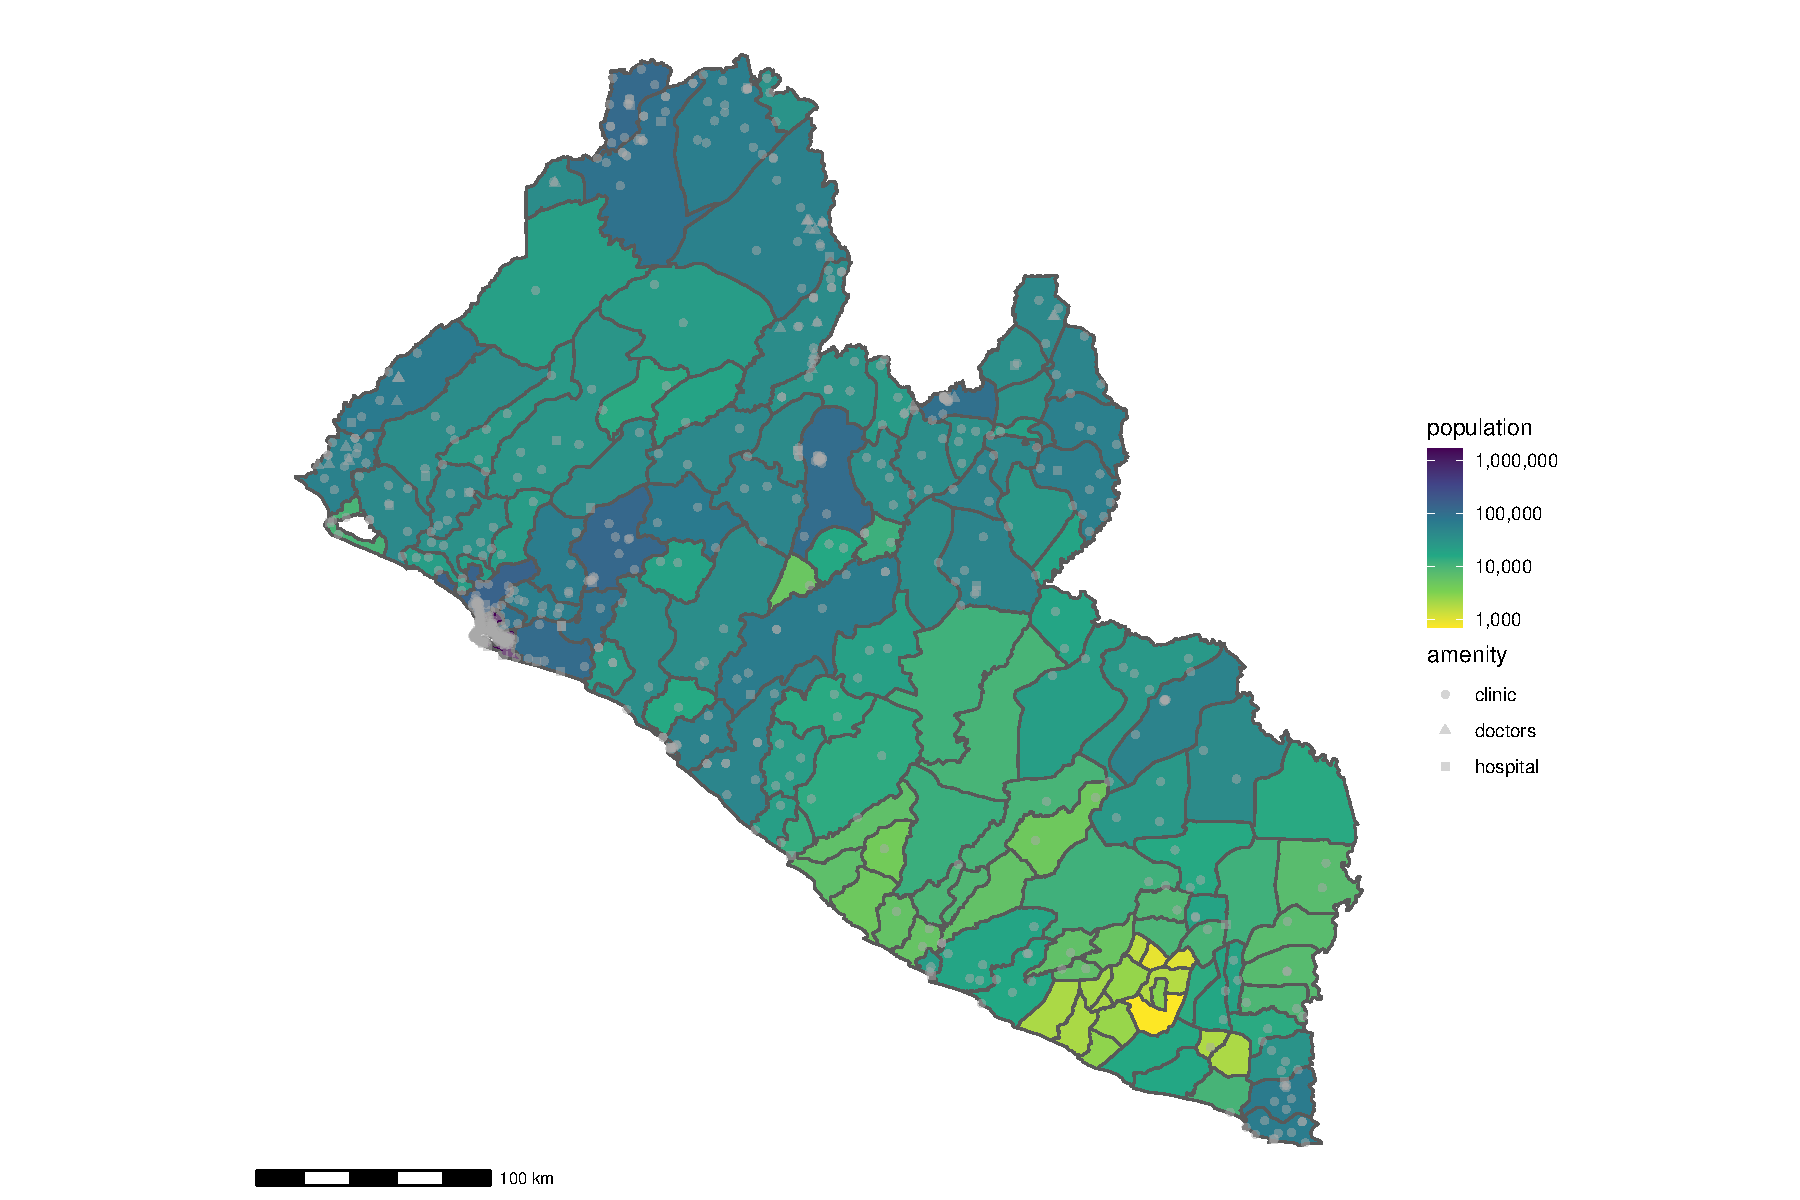
\includegraphics{_main_files/figure-latex/mappop-1.pdf}
\caption{\label{fig:mappop}Estimated population in 2021}
\end{figure}

\hypertarget{district-population-and-health-facilities}{%
\subsubsection{District population and health facilities}\label{district-population-and-health-facilities}}

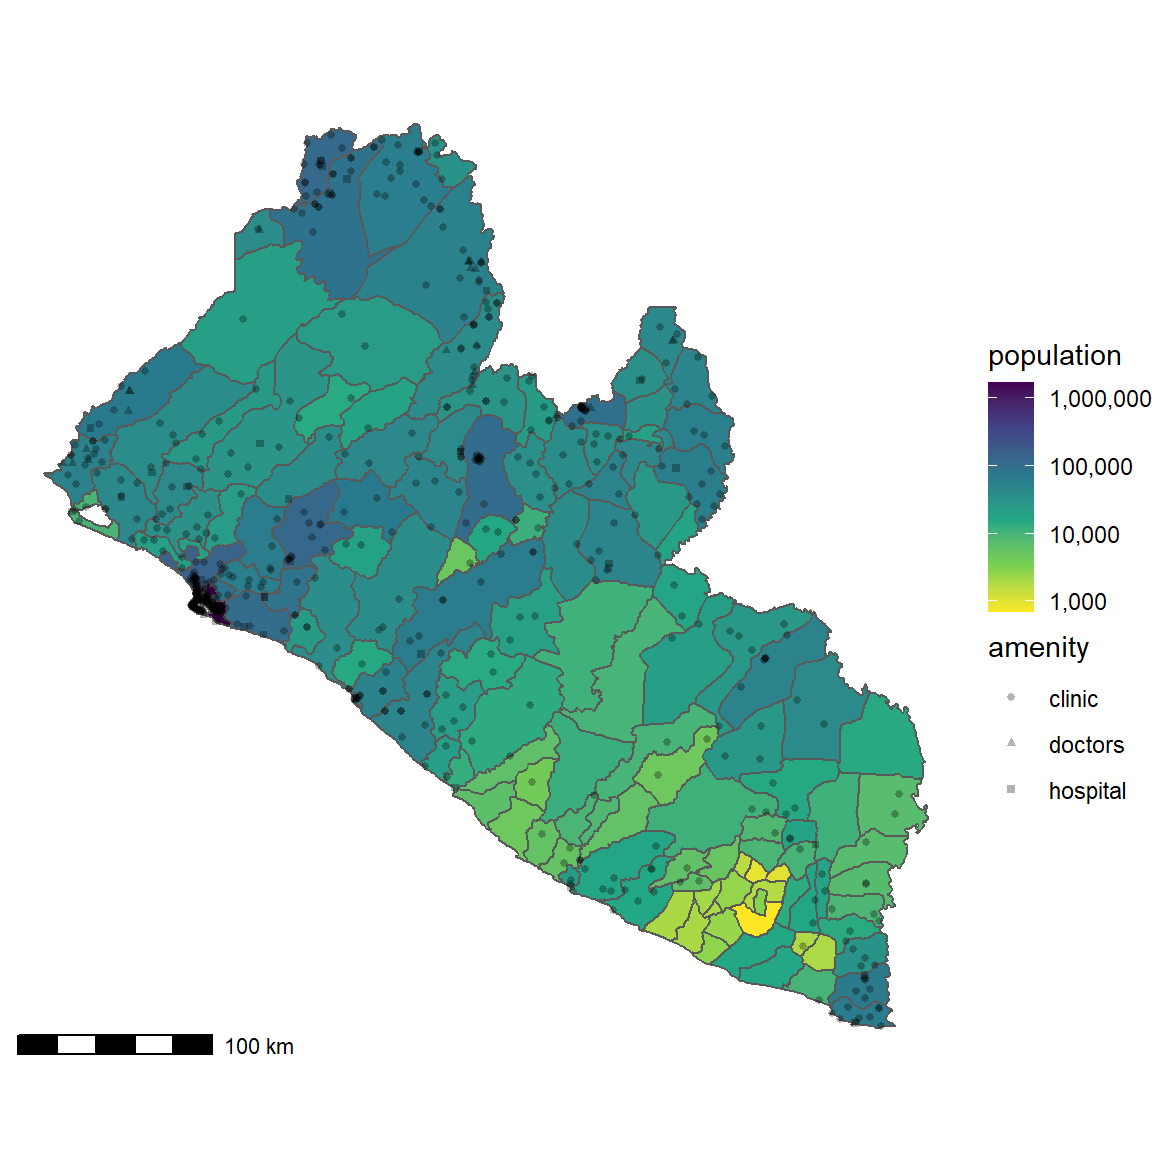
\includegraphics{_main_files/figure-latex/unnamed-chunk-2-1.pdf}

\hypertarget{district-population-density}{%
\subsubsection{District population density}\label{district-population-density}}

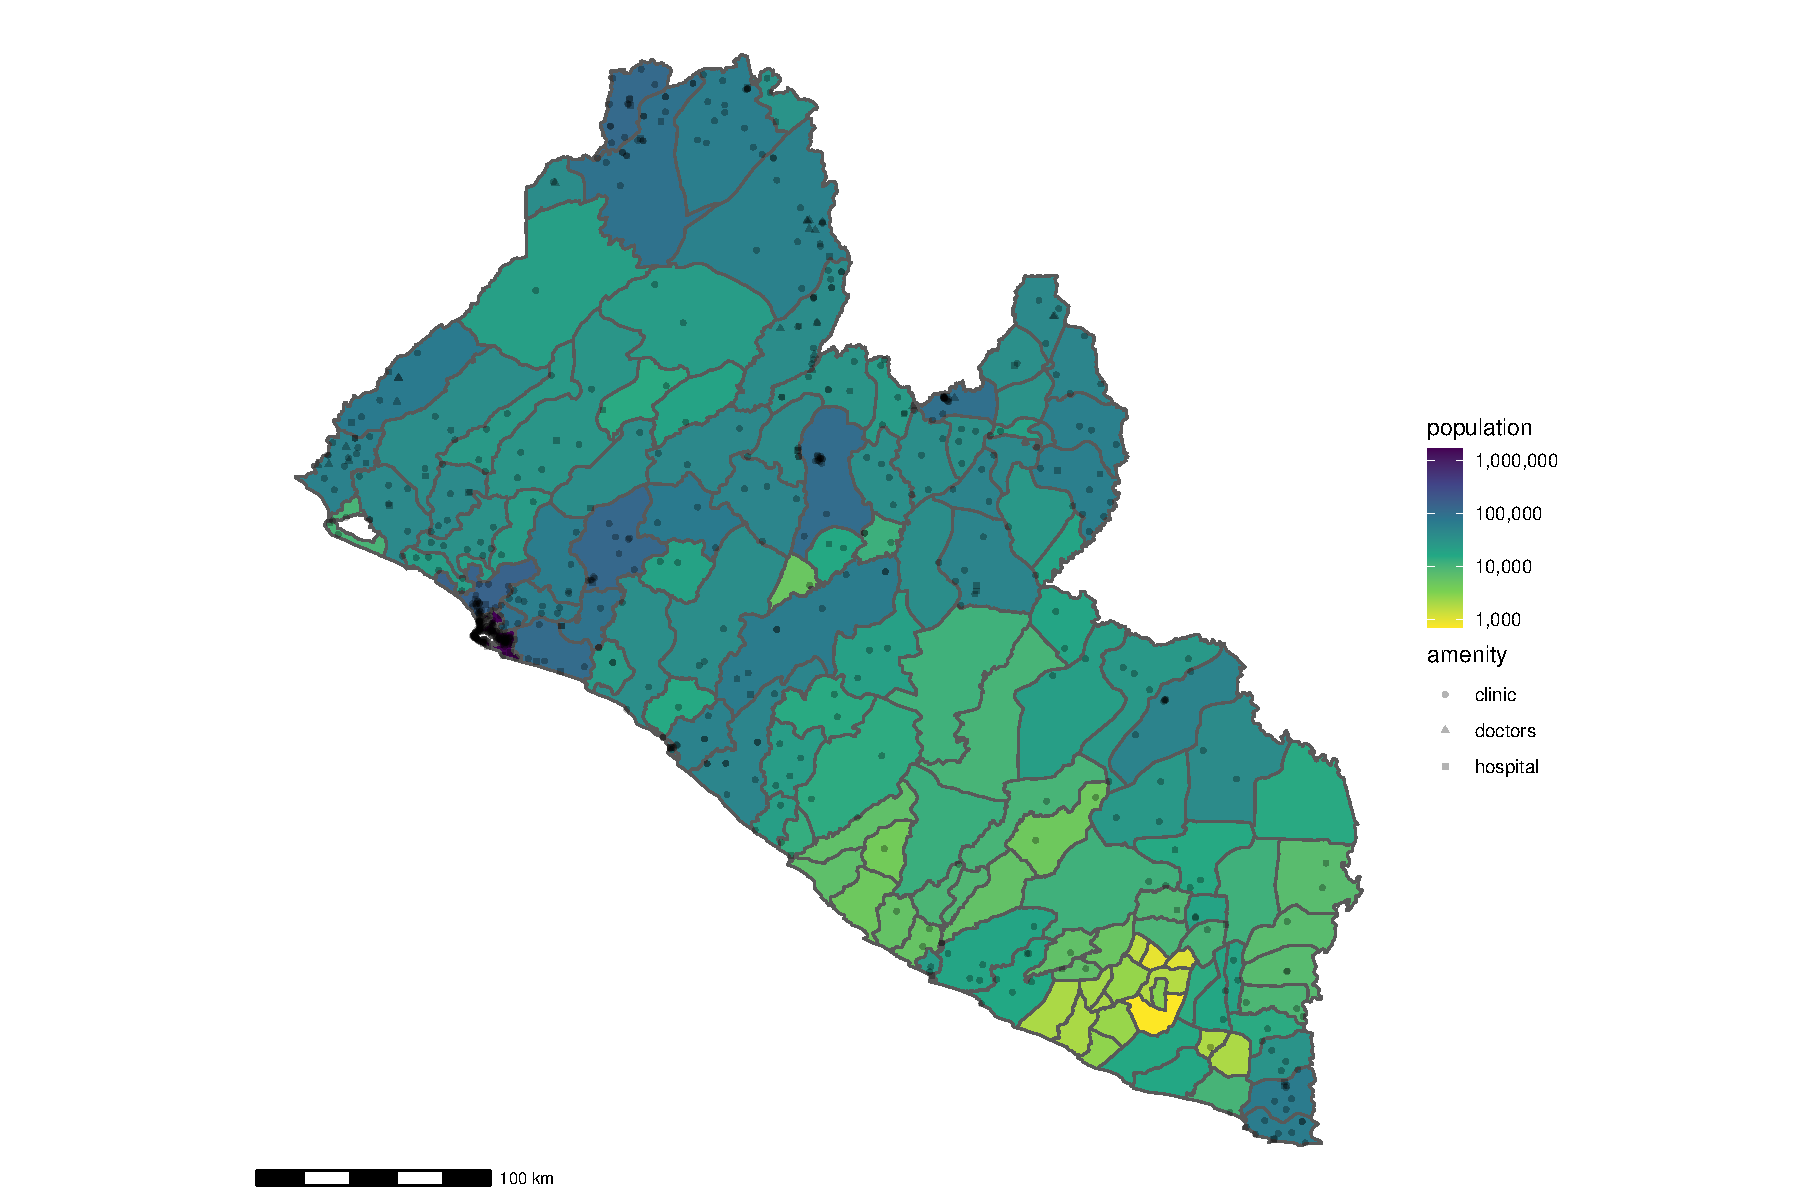
\includegraphics{_main_files/figure-latex/unnamed-chunk-3-1.pdf}

\hypertarget{land-distribution}{%
\subsubsection{Land distribution}\label{land-distribution}}

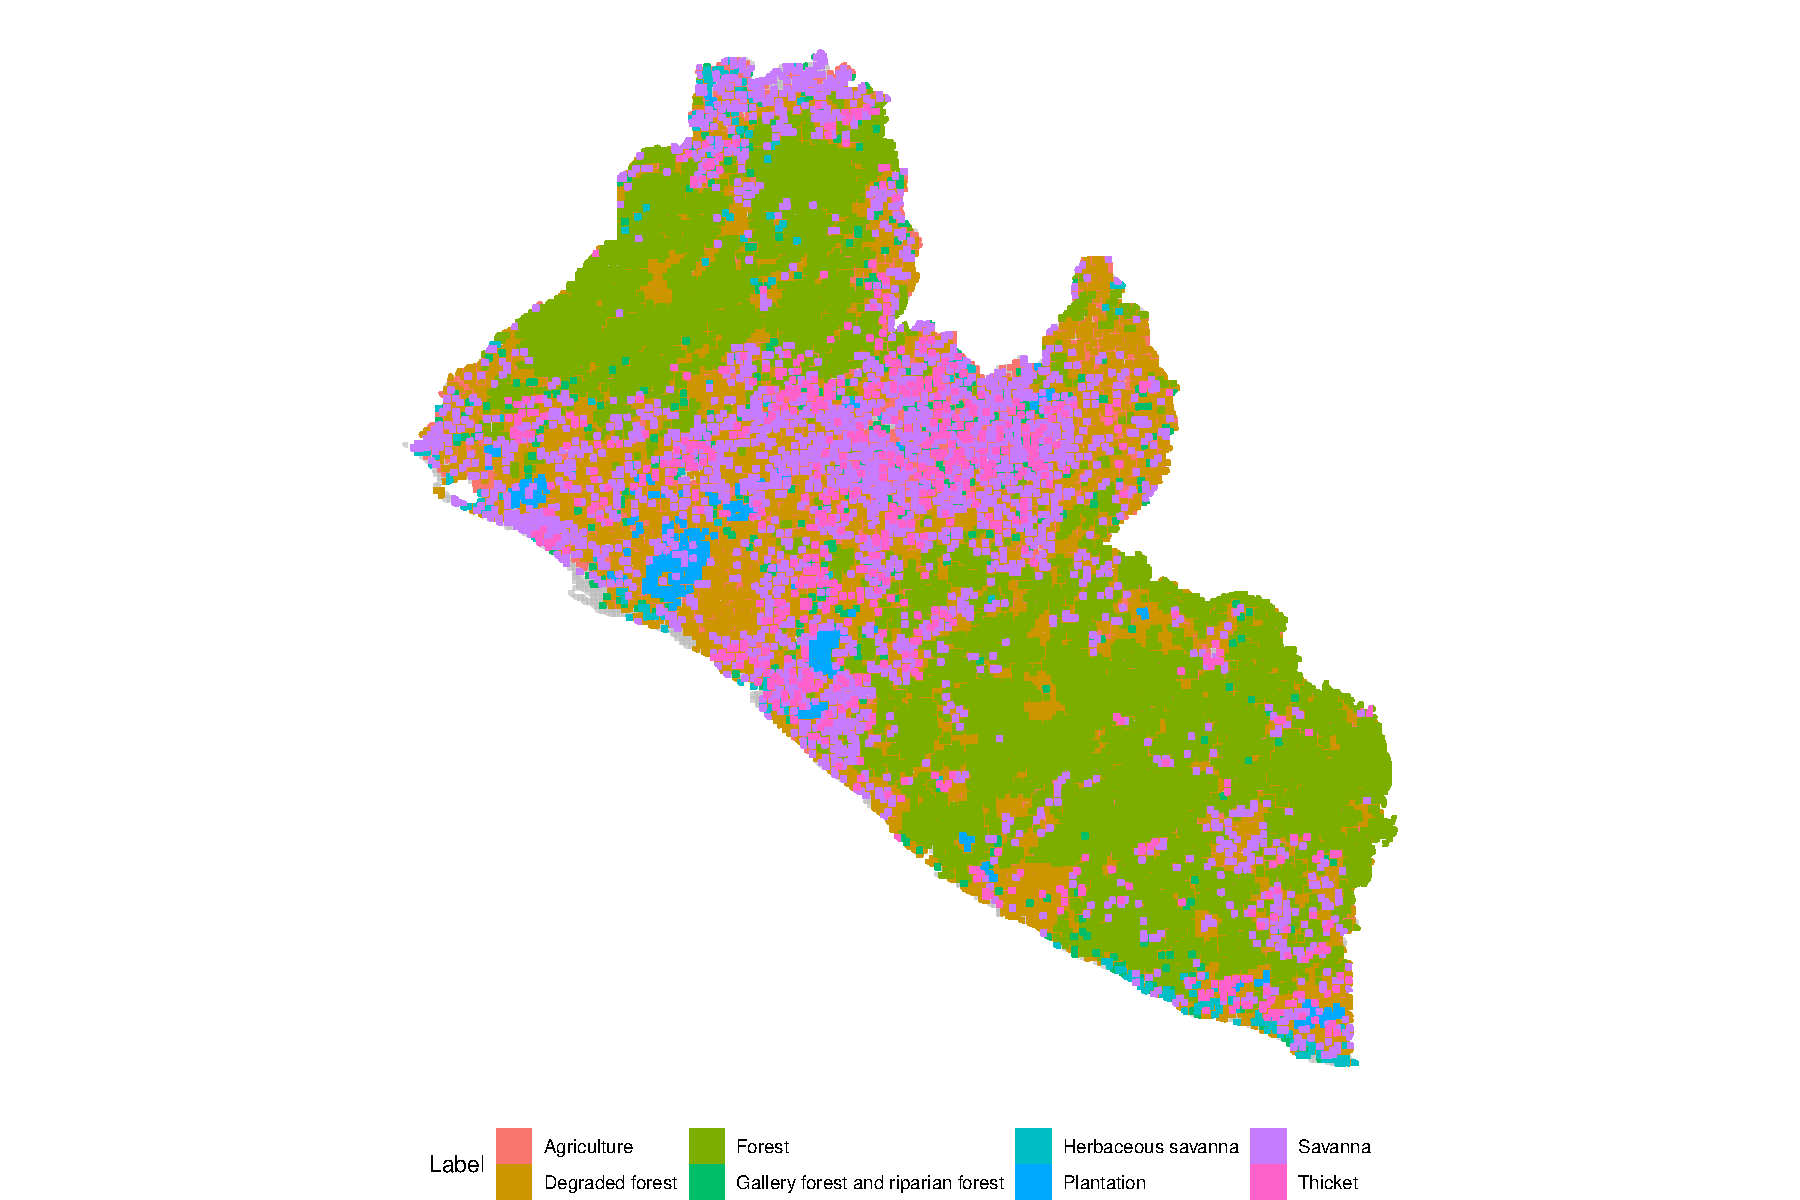
\includegraphics{_main_files/figure-latex/land-1.pdf}

\hypertarget{rivers}{%
\subsubsection{Rivers}\label{rivers}}

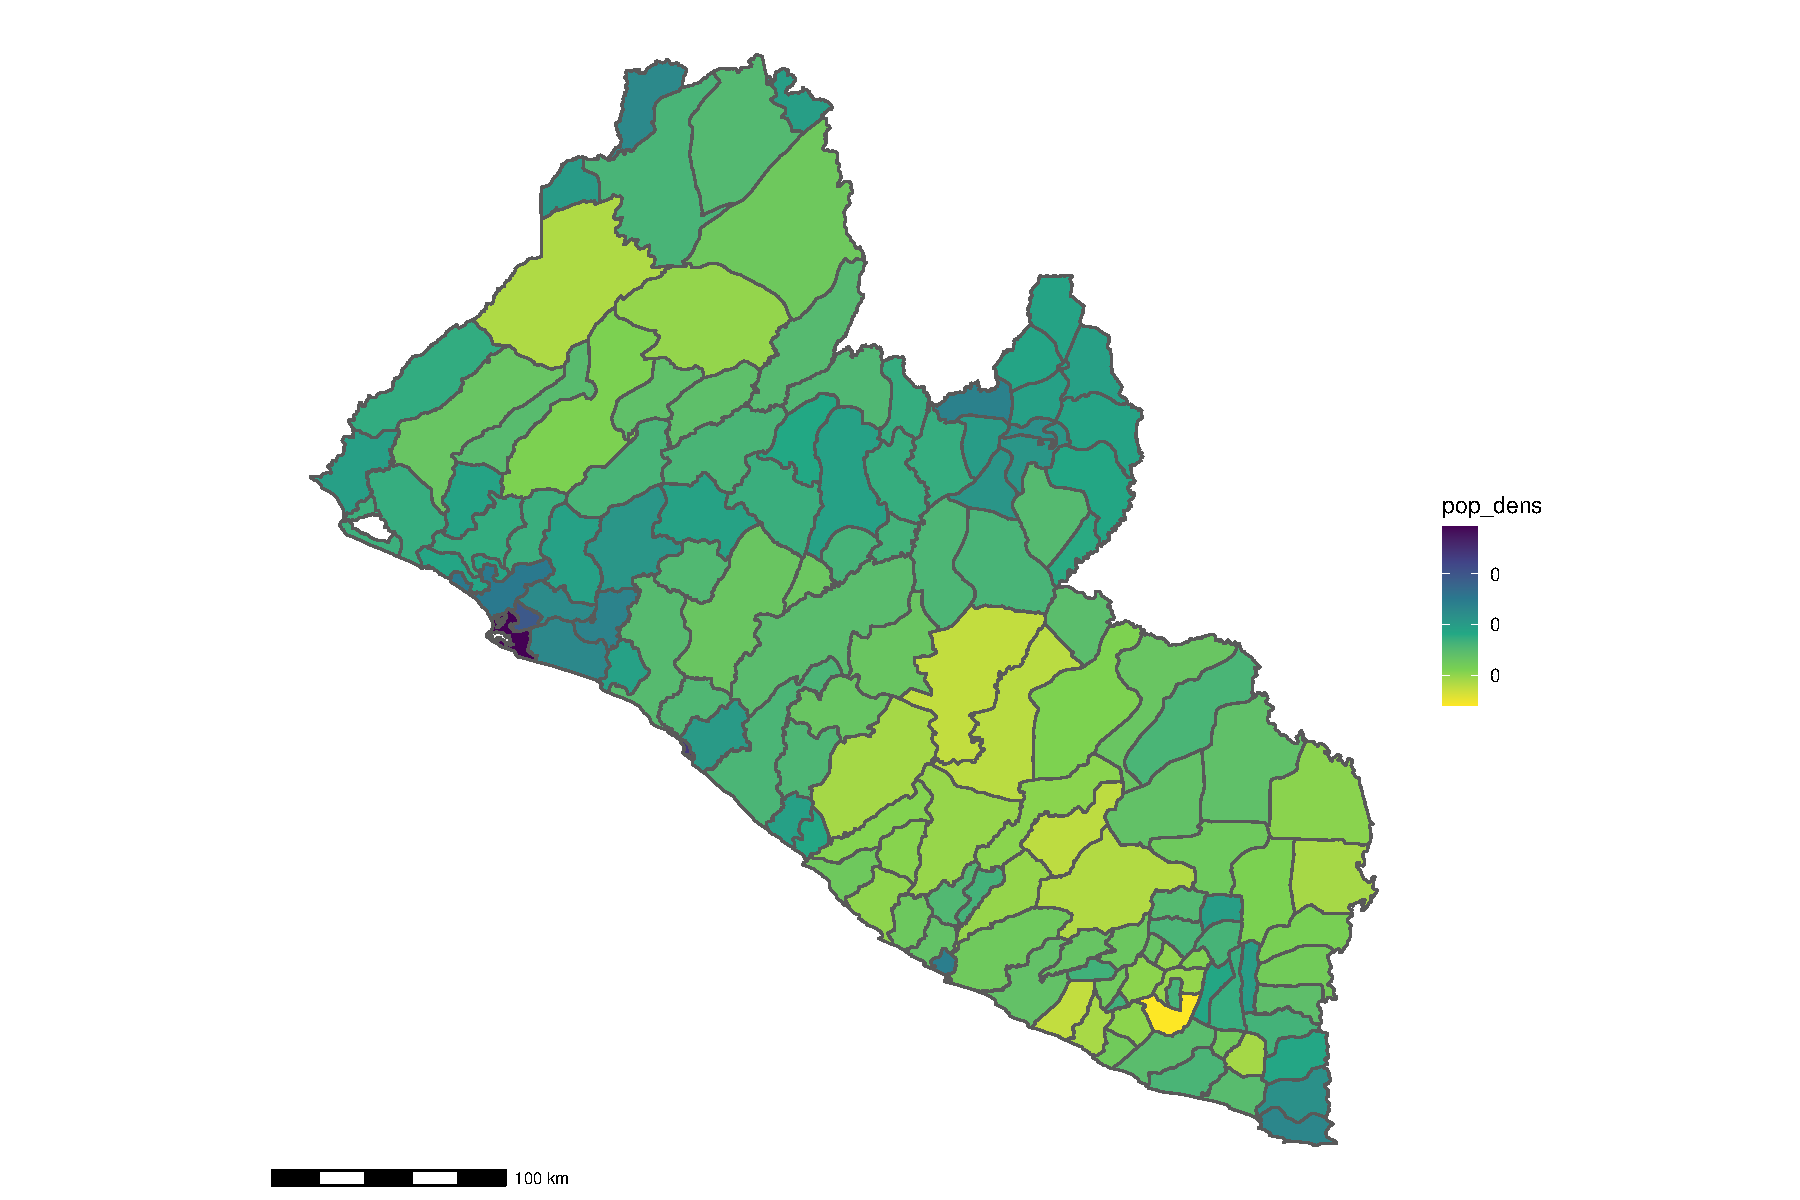
\includegraphics{_main_files/figure-latex/unnamed-chunk-4-1.pdf}

\hypertarget{bioclimate-variables}{%
\subsubsection{Bioclimate variables}\label{bioclimate-variables}}

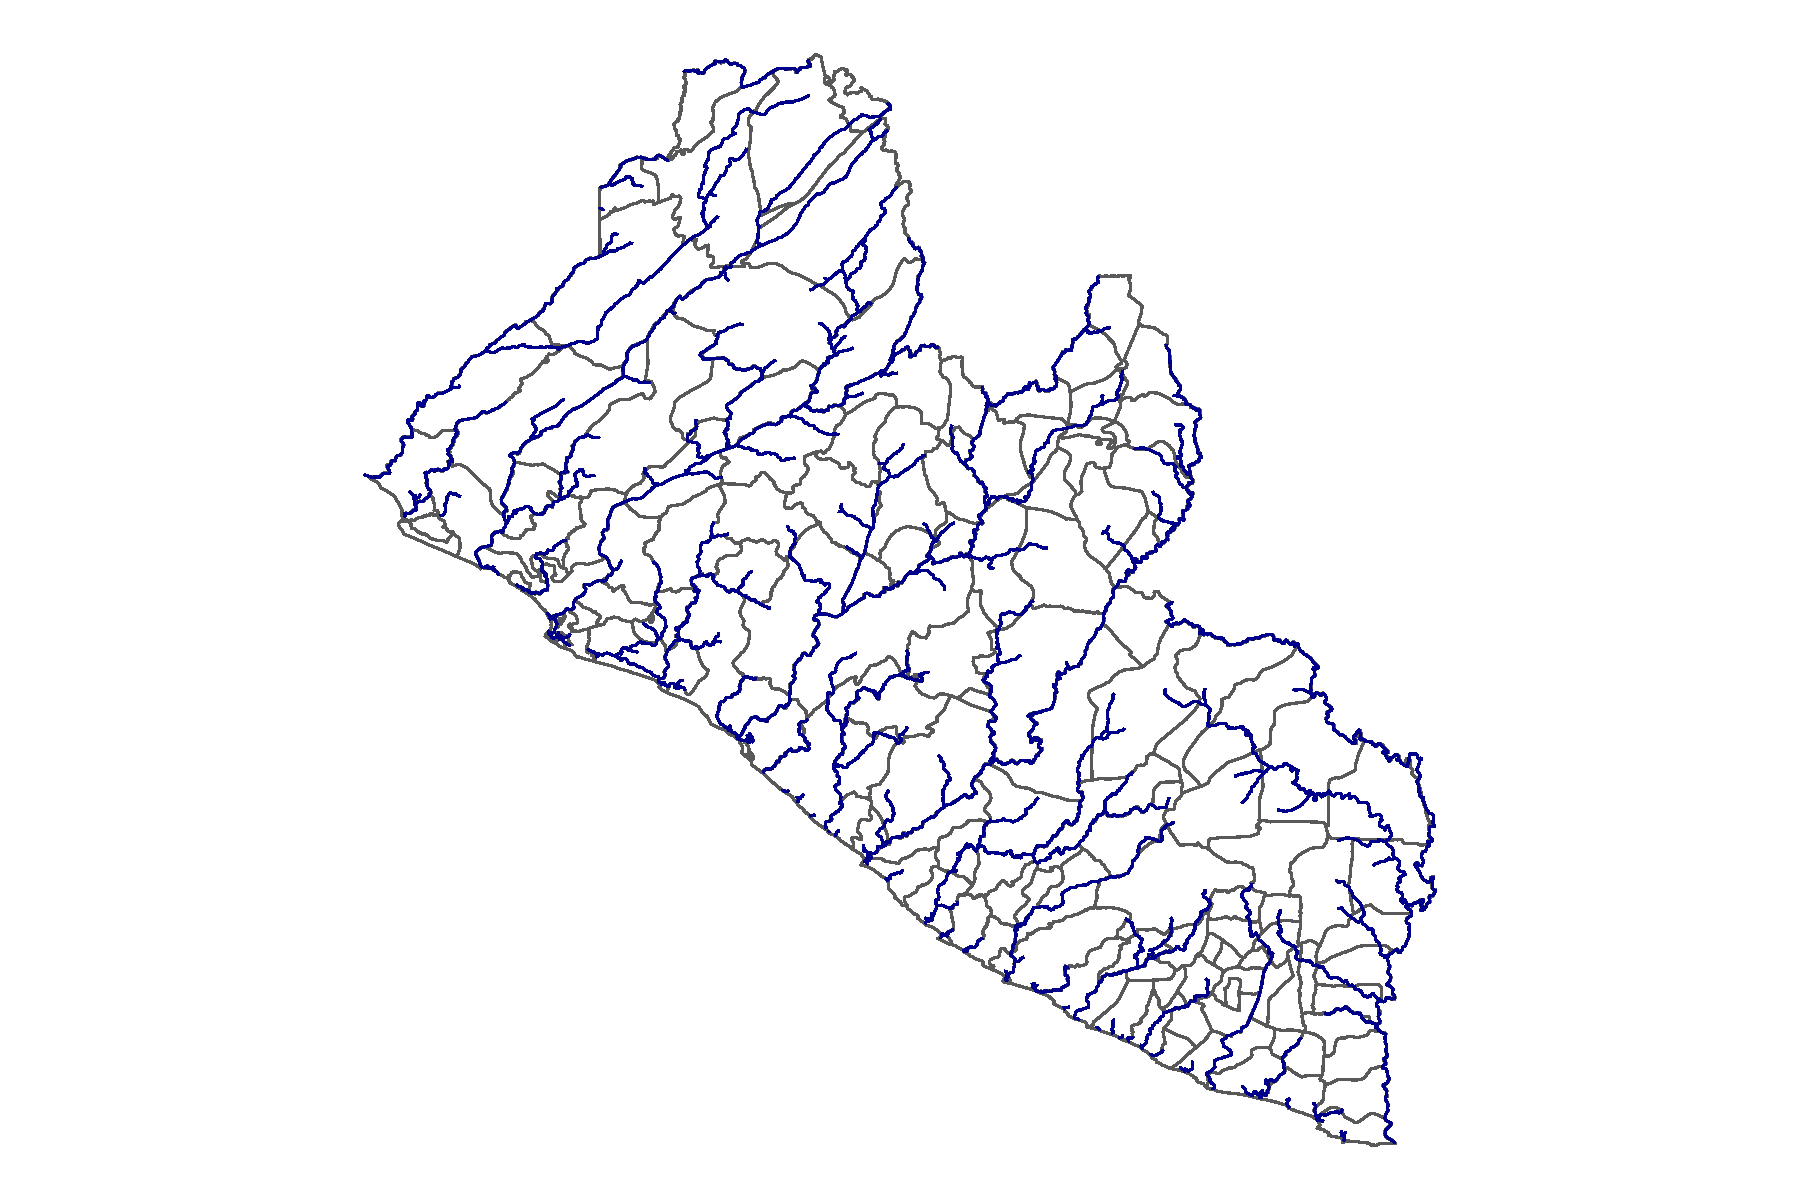
\includegraphics{_main_files/figure-latex/unnamed-chunk-5-1.pdf}

\hypertarget{refs}{}
\begin{CSLReferences}{1}{0}
\leavevmode\vadjust pre{\hypertarget{ref-cromwell2020}{}}%
Cromwell, Elizabeth A, Chris A Schmidt, Kevin T Kwong, David M Pigott, Denise Mupfasoni, Gautam Biswas, Shreya Shirude, et al. 2020. {``The Global Distribution of Lymphatic Filariasis, 2000{\textendash}18: A Geospatial Analysis.''} \emph{The Lancet Global Health} 8 (9): e1186--94. \url{https://doi.org/10.1016/s2214-109x(20)30286-2}.

\leavevmode\vadjust pre{\hypertarget{ref-mitjuxe02015}{}}%
Mitjà, Oriol, Michael Marks, Diby J P Konan, Gilbert Ayelo, Camila Gonzalez-Beiras, Bernard Boua, Wendy Houinei, et al. 2015. {``Global Epidemiology of Yaws: A Systematic Review.''} \emph{The Lancet Global Health} 3 (6): e324--31. \url{https://doi.org/10.1016/s2214-109x(15)00011-x}.

\leavevmode\vadjust pre{\hypertarget{ref-simpson2019}{}}%
Simpson, Hope, Kebede Deribe, Earnest Njih Tabah, Adebayo Peters, Issaka Maman, Michael Frimpong, Edwin Ampadu, et al. 2019. {``Mapping the Global Distribution of Buruli Ulcer: A Systematic Review with Evidence Consensus.''} \emph{The Lancet Global Health} 7 (7): e912--22. \url{https://doi.org/10.1016/s2214-109x(19)30171-8}.

\leavevmode\vadjust pre{\hypertarget{ref-who_global_2016}{}}%
WHO. 2016. {``Global Leprosy Update, 2016: Accelerating Reduction of Disease Burden.''} 92. \url{https://www.who.int/publications-detail-redirect/who-wer9235}.

\end{CSLReferences}

\end{document}
